\chapter{Methodology} % Main chapter title

\section{Complex networks}

Many real systems are composed of a large number of elements interacting with each other. Due to interactions, without any central force, the system exhibits the emergence of collective behaviour on the macro level. Such a system is called a Complex System and its properties can not be predicted from the behaviour of the one individual. An example of a complex system is the human brain. The structure of the brain network and its properties are fundamental for brain functioning, while an emergent phenomenon is a human intelligence. In societies, people's interactions lead to civilization, economy, formation of social groups. Also, the animal populations show different levels of organization that emerge from the individual's interactions \cite{boccaletti2006complex}. %latorro

The research in complex systems focuses on the structure of the interactions between units. Knowing how branches of the system are connected, we can determine the emergence of the collective behaviour of the system. For the brain network, we can construct representation with neurons and synapses, representing the brain connectivity. Neurons in the same brain area are closely connected \cite{latora2017complex}. Similarly, we can define communication between people. The structure of these interactions gives us insights, for example, how information propagates through the system. The presence of people with many connections can lead to faster information flow. 

Despite the differences between complex systems, they can be studied using complex networks; with sets of nodes (vertices) and links (edges). Elements in the system are nodes, while interactions between them are given as edges. This approximation allows us to treat equally social (graph of actors), biological (network of proteins) or even technological systems (internet, traffic) \cite{costa2007characterization, costa2011analyzing}.  In recent years, complex network theory has application in different fields, and the availability of big data incurs its development.
%Analyzing and Modeling Real-World Phenomena with Complex Networks: A Survey of Applications
%Characterization of Complex Networks: A Survey of measurements

The complex network theory originates from the graph theory in mathematics. %These days, the graph and network are used as equivalent terms. 
The first mathematical problem solved using graph theory was $Konigsberg$ problem of seven bridges. The city $Konigsberg$ had seven bridges connecting the city's parts across the river and the island in the middle. The question was, is it possible to find a walk that crosses all seven bridges only once. Representing the problem as a graph, as in figure \ref{fig:Krgraph}, Euler managed to simplify the problem; the parts of the land are represented as nodes while bridges between them are links. Crossing each bridge only once is possible if each part of the land has an even number of connections. By this it is possible to enter one part of the land from one bridge and leave it by the other. As each node has odd number of connections, in this case it is not possible, see Fig. \ref{fig:Krgraph}.

\begin{figure}[h!]
	\centering
	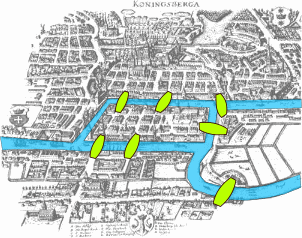
\includegraphics[width=0.3\linewidth]{Figures/Konigsberg_bridges.png} \hspace{2cm}
	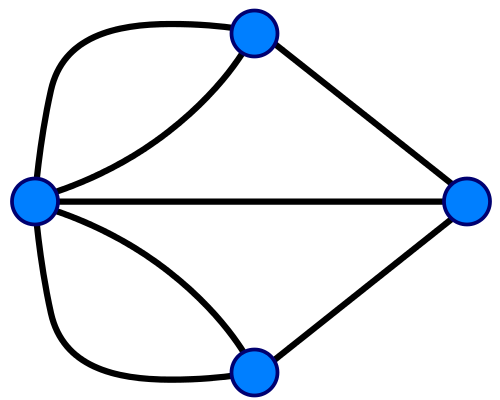
\includegraphics[width=0.3\linewidth]{Figures/Konigsberg_graph.png}
	\caption{The Kronigsber problem of seven bridges.}
	\label{fig:Krgraph}
\end{figure}

\section{Types of networks}

The graph or network $G$ is defined as $G=(\boldsymbol{V}, \boldsymbol{E})$, where $\boldsymbol{V} = \{ v_1, v_2, ... v_N\}$ is a set of $N$ nodes (vertices), and  $\boldsymbol{E} = \{e_1, .. e_L\}$ is a set of $L$ edges (links). The edge is pair of nodes $e = (v_i, v_j), $ such that $\{v_i,v_j\}\in \boldsymbol{V}$. The most basic network representation considers \textbf{unweighted and undirected} structure. The edges are unweighted, meaning that all interactions in the network are equally important.  Because network is un-directed, edges are symmetric, such that $(v_i, v_j)$ implies $(v_j, v_i)$. In \textbf{directed} networks this simmetry is broken. The interaction between two nodes $v_i$ and $v_j$, can be only in one direction. A typical example is World Wide Web, where webpages are nodes and hyperlinks are directed edges. In biological networks, gene regulation and neural activation can be described as directed network. The first column a) in Figure \ref{fig:graph_dir} shows the graphical representation of two networks with equal number of nodes; the first one is underected and the second one is directed. 

Even though, graphical representation can be useful for describing the network structure, mathematical representation allow us to characterize the statistical properties of the networks. The graph $G$, with $N$ nodes could be represented with \textbf{adjacency matrix} $|A| = N \times N$ \cite{boccaletti2006complex}. The elements of the matrix are positive if there is connection between two nodes $v_i$ and $v_j$. 
\begin{equation}
A_{ij} =
\begin{cases}
1 & \text{ ($v_i$, $v_j$) $\in$ $E$}\\
0 & \text{ ($v_i$, $v_j$) $\notin$ $E$}
\end{cases}       
\end{equation}

The column b) on Figure \ref{fig:graph_dir} shows adjacancy matrix representation of given graphs. By convention diagonal elements $A_{ii}=0$, as self-loops are not allowed. For undirected network adjacency matrix is symmetric $A_{i,j}=A_{ji}$, but in the case of directed network matrix is not symmetric, as edges are drawn in one direction only.  

\begin{figure}[h!]
\centering
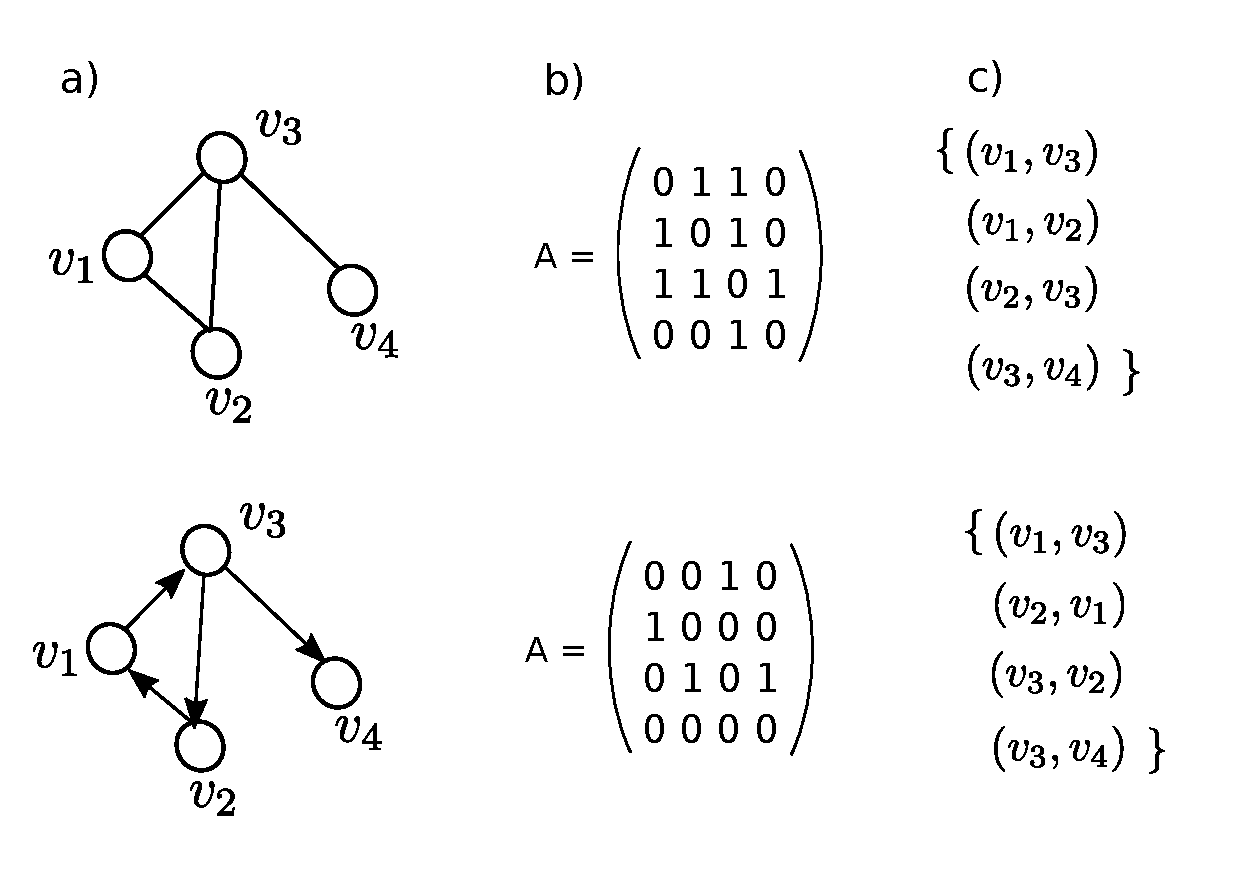
\includegraphics[width=0.7\linewidth]{figures/methodology/directed_graph.pdf} 
\caption{a) Graph representation of undirected (top panel) and directed (bottom panel) network. The same networks are represented with adjacency matrices column b), and edge list representation in column c).}
\label{fig:graph_dir}
\end{figure}

The number of edges and nodes are dependent variables. Considering that each node can make $N-1$ connections, the maximum number of the edges in the network is $L_{max}=N(N-1)/2$, as each edge is counted twice. For directed network it is possible to draw $L_{max}=N(N-1)$ edges \cite{caldarelli2007scalefree}. When it comes to large networks, they are sparse, meaning that the number of links is $L<<L_{max}$. As consequence, the adjacency matrix is also sparse structure (has many zeros) that takes large portion of computer memory \cite{barabasi2016network}. 
It is common to represent the graph as edge list. In this case, illustrated on Figure \ref{fig:graph_dir}, column c), graph is described with the list of links that are in the graph, $G = \{ \{v_i,v_j\}\}$. Still with this representation we are not able to distinguish between directed and undirected graph structures, so in the computational algorithm should be specified if the edges are considered symetric or not.  
%To distinguish between undirected and directed structures, for undirected representation it is possible writing two edges $(v_i, v_j)$ and $(v_j, v_i)$, otherwise in the computational algorithm should be specified if the edges are considered symmetric or not.

\begin{figure}[h!]
	\centering
	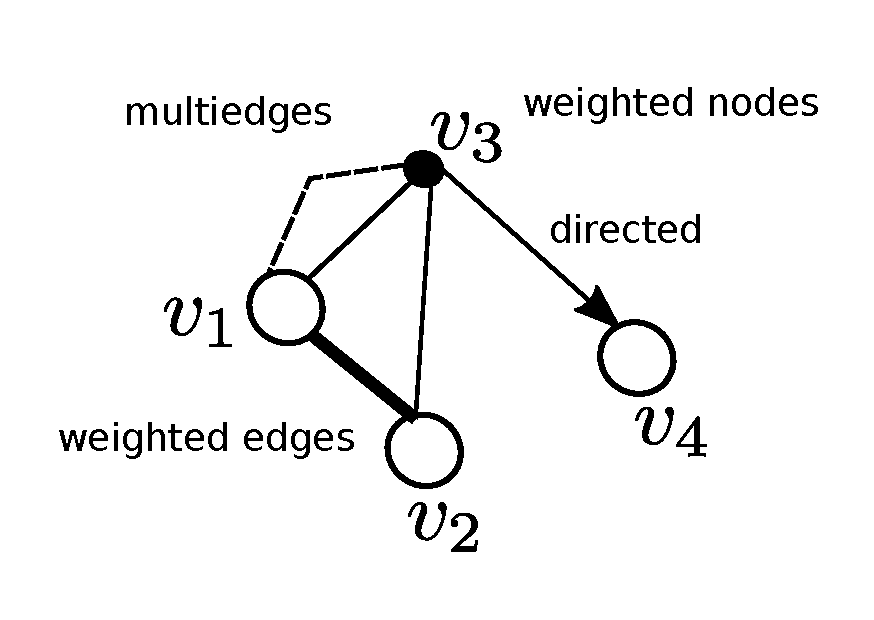
\includegraphics[width=0.4\linewidth]{figures/methodology/multi_graph.pdf} 
	\caption{The complex networks may represent different characteristics of the system. The edges can be directed, weighted or multiply. Also nodes can be assigned with different weights or any relevant feature.}
	\label{fig:multigraph}
\end{figure}

To create the more realistic models, sometimes is essential to include the specific properties of the system in the network representation. For example, to emphasis the frequent interactions between nodes, edges can be assigned with different values, such networks are \textbf{weighted}. They can be described with adjacency matrix, whose elements can take any real number $A_{ij}=w_{ij}$ and $w_{ij}>0$. In general edges may be associated with any categorical variable. Similarly additional properties can be added to nodes, or even to the whole network structure. To include the \textbf{temporal} component in the network, edges are characterized with the time when the interaction between nodes happen. Finally, if two nodes interact in different ways, the \textbf{multigraph} is appropriate configuration where multiply edges are allowed. The graphical representation of discussed network representations is given on the Figure \ref{fig:multigraph}. \\~\\
% the network between cities, edges may be different driving paths between them. In neuron cells, multiply synapses are represented as distinct edges. \\ %\cite{barabasi2016network, latora2017complex, newman2010}
A \textbf{bipartite network} consists of two types nodes. The nodes in the same partition are not connected, while links exist only between partitions. For many real systems, a bipartite graph is a natural representation\cite{barabasi2016network, latora2017complex}. For example, the bipartite network of people and groups has two distinct node partitions while links indicate the memberships. Another example is a system of customers and products. The link between user and item is created when the user buys an item. The bipartite networks find their application in the algorithms for recommended systems, whose goal is to recommend items that may interest the user. Actually, to find the most probable missing links in the network. 

In a bipartite network, nodes in one partition are not connected. Still, we can analyse a single node type if we project the bipartite network on one partition. The primary assumption is that two nodes in one partition could be connected if they point to the same node in another partition. Consider the network of movies and actors. The one mode projection of movies is an undirected network whose links indicate that two movies share the same actors. On the other hand, another projection is a network of actors. The links exist if two actors appear in the same movie \cite{newman2010, barabasi2016network}.

\begin{figure}[h!]
	\centering
	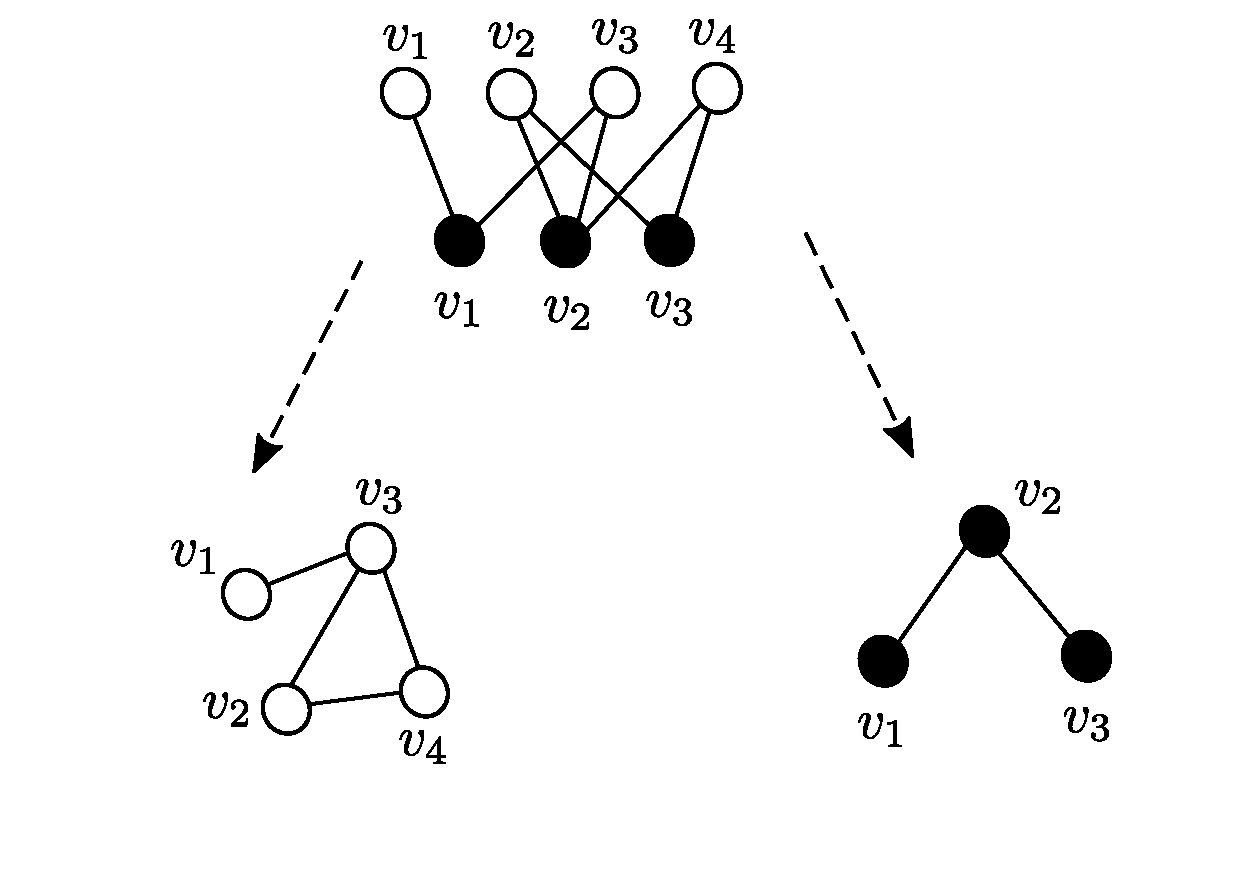
\includegraphics[width=0.7\linewidth]{figures/methodology/bipartite_graph.pdf} 
	\caption{Bipartite graph and two partition projections.}
	\label{fig:gt2}
\end{figure}

We should be aware that important information is lost when creating a one-mode projection. First of all, without having weighted edges in the network of actors, it is impossible to have information on how many movies two actors appear in. From the one-mode projection, we can not reconstruct the original network. Moreover, two different bipartite networks may have the same projected networks. The important consequence of the network projection is the creation of cliques; subgraphs where all nodes are connected. 

In general, it is possible to define the k-bipartite network. The same rules apply as before. There are $k$ distinct node partitions, while the edges exist only between different types of nodes.\\



%The product $B_{ki}$ and $B_{kj}$ is 1 if $i$ and $j$ belong to the same group $k$. Thus the total number of groups to which nodes $i$ and $j$ belong is $P_{ij} = \sum_{k=1}^g B_{ki}B_{kj} = \sum_{k=1}^g B_{ik}^TB_{kj}$. The matrix $P$ is matrix of one-mode projection. The diagonal elements are non-zero, and represent the number of groups node $i$ belongs to.  To derive the weighted adjacency matrix, the diagonal elements are set to 0. The adjacency matrix of unweighted projection, each non-zero element needs to be replaced with $1$. 

\textbf{Temporal networks.}
Studying the real systems as static networks can give us a lot of insight into the system properties. Still, real systems are not static; they evolve not only in the number of elements but also in the number of interactions between them. Some interactions in the system may repeat in different intervals and could be described with complex activity patterns. Including time dimension in the network representation allows us to study the properties of the system closely. The temporal information may matter a lot \cite{holme2012}. For example if interaction between nodes $(v_1, v_2)$ happened before in time than  $(v_2, v_3)$, then nodes $v_1, v_3$ would not be connected, as it is the case in the static network. 

The temporal network is a collection of timestamped edges. Each edge is defined as $(v_i, v_j, t, \Delta t)$, where $v_i$ and $v_j$, are nodes $t$ is time when interaction happen, and $\Delta t$ is event duration \cite{guide_temporal}. The duration of the events may vary, as in the phone-call network. Also, for many systems, the time resolution of event duration is too small. For example, this parameter may be neglected when people interact on social platforms or email each other because the event time is too short, it scales in seconds.

\begin{figure}[h!]
	\centering
	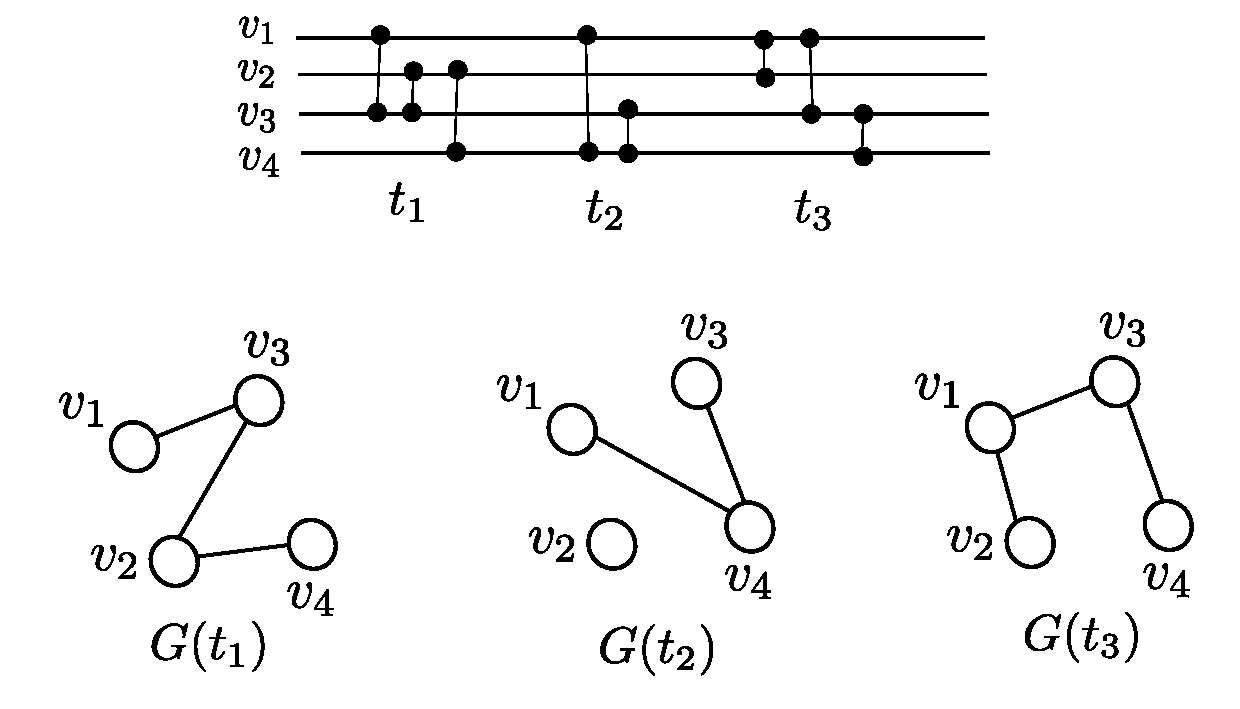
\includegraphics[width=0.7\linewidth]{figures/methodology/temporal_network.pdf} 
	\caption{Temporal network. }
	\label{fig:gt3}
\end{figure}

The temporal network can be represented as sequence of static networks that evolve in time, $G = \{ G(t_1), G(t_2), ..., G(t_{max})\}$. At each time step, we can create the network and analyze the macroscopic properties of the given network snapshot. With this, we can end up with graph snapshots with many disconnected components or empty graphs for some points \cite{holme2015modern}. Sometimes, a much better approach is to aggregate the links that over time-windows. Here, we need to specify the time window length $w$. Interactions in the time interval $0\leq t<w$ enter the first snapshot. The next snapshot takes edges $w \leq t <2w$, and so on. The time windows are not overlapping, but generally, it is possible to slide the time window for different periods $ 1 \leq \delta t \geq w$. The downside of this method is that we can not recover original data points. The larger the time window is, the more information is lost. If the time window is set to $w=t_{max}$, there is only one snapshot, and the temporal data are no more available \cite{krings2012effects, arnold2021moving}. \\

\textbf{Multilayer networks} were introduced for studying systems in which different types of interaction exist. This formalism allows one to investigate diverse network systems and to combine different types of data into one model \cite{porter2018multilayer}. In a multilayer or multiplex network, all nodes are present in each layer, but their interactions among layers differ. Two nodes may be connected in one layer but not in the other. Different online social systems may be an example of a multiplex network when users are connected on one platform but not on the other \cite{aleta2019multilayer}. Or the airline transportation network, where each layer represents the flights of different airline companies \cite{kivelamultilayer}.   

%Consequently, we can partition the set of links into intralayer links, that is, links that connect nodes set in the same layer, and interlayer or coupling links, which are those links that connect nodes set in different layers. 

%A temporal network is a special kind of multiplex network, where these layers form a temporal (ordered) sequence. Crucially, there can dynamics on each vertex that govern which layer some kind of interaction occurs on, so multiplex networks are not merely a special kind of graph in which different colors or layer numbers annotate edges. %clauset preformulisati

%\subsection{Multigraphs}
%\begin{figure}[h!]
%	\centering
%	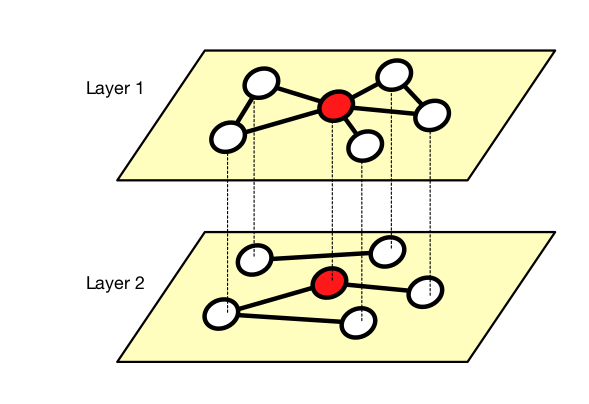
\includegraphics[width=0.5\linewidth]{figures/methodology/graph5.png} 
%	\caption{Graph types}
%	\label{fig:gt5}
%\end{figure}

%Spatial networks are a special kind of node-annotated network, in which the annotations represent the node's location in some d-dimensional space. This graph property is most common in transportation networks, e.g., as road and city networks, airport transportation networks, oil and gas distribution networks, shipping networks, etc., but can also appear in social networks. Planar graphs are a special case of spatial networks in which the nodes are embedded on a 2-dimensional surface and edges do not cross. %clauset preformulisati

%Hypergraphs are another type of network, in which edges denote the interaction of more than two vertices, e.g, E in V × V × V . Scientific collaboration graphs can be represented as a hypergraph, in which each "edge" is the set of coauthors on a scientific article. However, collaboration networks are more commonly represented as bipartite graphs, in which scientists and papers form two sets of vertices, and scientist-nodes are connected to all the paper-nodes on which they are authors. %clauset to do

%The canonical network form is an undirected graph, where two nodes are either connected or not. This applies to situations where two nodes are either in a relationship with each other or not, but it cannot be that one is related to the second without the second being related to the …rst. This is generally true of many social and/or economic relationships, such as partnerships, friendships, alliances, acquaintances, etc. This sort of network will be central to most of the chapters that follow. However, there are other situations that we will examine that are better modeled as directed networks, where one node may be connected to a second without the second being connected to the …rst. For instance, a network that keeps track of which authors cite which other authors, or which web pages have links to which others would naturally take the form  of a directed graph.

\section{The structure of complex networks}

%The complex system can be represented by complex network $G=(V, E)$, where the elements of system (atoms, proteins, people) map to set of $N$ nodes $V=\{1, 2, ...,N\}$. The interactions between elements map to $L$ links between nodes, $E = \{ e_1, e_2... e_L\}$. The \textbf{adjacency matrix} ${A} = N \times N$ has value $1$ if there is connection between two nodes, otherwise it is $0$ \cite{boccaletti2006}. 

\subsection{Degree distribution}

The simplest network measure is \textbf{node degree}, $k$. The degree of node $i$ gives the number of nodes attached to node $i$, $k_i = \sum_j A_{ij}$. 

The density of the network is average degree divided by $N-1$, where $N$ is number of nodes. It is relative fraction of nodes in the network. 

In the case of regular networks, such as grids, each node has an equal degree, meaning that nodes in the network have similar roles. In the general case, the networks have more complicated structure. If degree sequence is skewed, we are able to identify nodes with high degree, hubs. Removing hubs may partition a connected network into several components. Finally, if we are able to test isomorphism between two graphs, the starting point would be to compare their degree sequences are the same. If they are not same, then graphs can not be isomorphic. \\

To calculate the degree distribution we can consider the fraction of $k$ degree nodes $N_k$, $p(k) = N_k/N$. It is the probability , $P(k)$, that randomly chosen node has degree $k$. Similarly, we can order nodes according to their degree and plot the node degree. \\
%If degree distribution is present $P(k)$, and the total number of nodes is fixed to $N$. We can construct a graph with random connections. Label N vertices. To node $j$ of the graph ascribe degrees $k_j$, taken from the distribution $P(k)$. Connect at random ends of pairs of distinct quills belonging to distinct vertices. 

If the nodes of the graph are statistically independent, the degree distribution completely determines the properties of a network. Here we summarize the forms of degree distributions that are mostly found in the complex network theory:
\begin{itemize}
	\item The Poisson distribution. The degree distribution in random network, where all nodes have the same connecting probability, follows Poisson distribution $P(k)= \frac{(Np)^ke^{-Np}}{k!}$, where $k$ is the mean degree distribution. 
	
	\item Exponential distribution. $P(k) = e^{-k/ \- k}$. This is degree distribution of the growing random graph. Even for infinite networks all moments of distributions are finite, and have natural scale of the order of average degree.
	
	\item In many real networks degree distribution follows a power law. $P(k) = k ^ {-\gamma} $, where $\gamma$ is exponent of the distribution. In this distribution there is no natural scale, so they are called scale-free networks. In infinite networks all higher moments diverge. If the average degree of scale-free networks is finite, than $\gamma$ exponent should be greater than 2. Therefore, real networks have a scale-free structure with the emergence of the hubs \cite{newman2010}. In finite size networks, fat-tailed degree distributions have natural cut-offs. 
\end{itemize}

 \begin{figure}
 	\centering
 	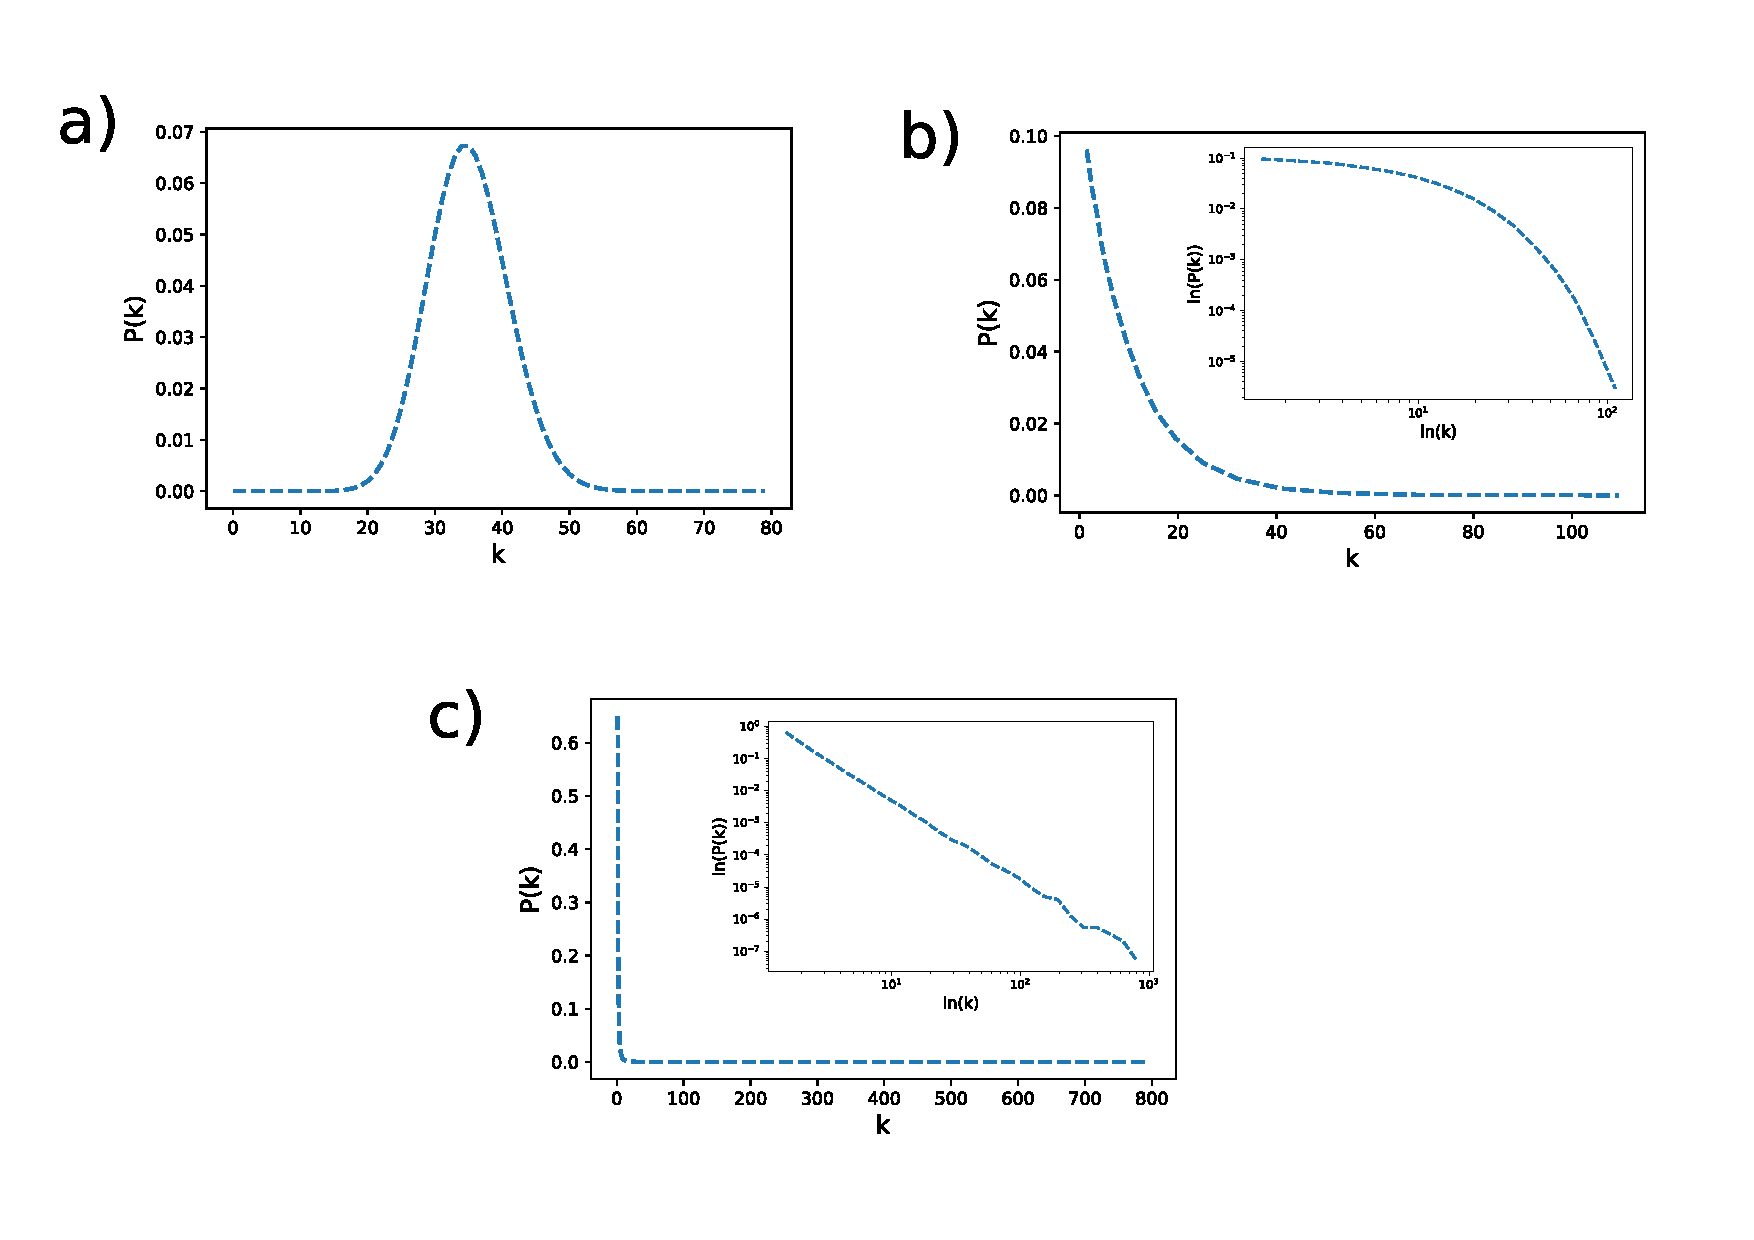
\includegraphics[width=0.7\textwidth]{codes/test1.pdf}
 		%figures/methodology/distributions.png}
 	\caption{Distributions, ovde hocemo 3 distribucije+ linearna vs. logarithm scala, takodje pokazati kako izgleda frequency order}
 	\label{fig:dist}
 \end{figure}

When plotting the degree distribution, it is common to use scaling of the axis. We rank the nodes according their degree and plot the node degree of each k-th node. As many nodes have  low degree, like for power-law or exponential distribution it is more useful to use logarithmic scale. Now it is more easily notices that data-points follow straight line, meaning that degree distribution is some kind of exponential function. 

%On the logarithmic scale the distance between two points is proportional to the logarithm of distance between two points, meaning that distance on logarithm scale is same between points 10 and 100, and 100 and 1000.  

\subsection{Degree correlations}

Correlation is defined through a correlation coefficient r. If x and y are two stochastic variables, for which we have a series of observation pairs $(x_1, y_1), (x_2, y_2), ... (x_n, y_n)$. The correlation coefficient $r(x, y)$ between $x$ and $y$ is defined as:

\begin{equation}
r(x, y) = \frac{\frac{1}{n}\sum_{i=1}^{n}((x_i - \bar{x} ) (y_i - \bar{y}) )}{\sqrt{\frac{1}{n}\sum_{i=1}^{n}(x_i - \bar{x})^2} \sqrt{\frac{1}{n}\sum_{i=1}^{n}(y_i - \bar{y})^2} }
\end{equation}

where $\bar{x} = \frac{1}{n}\sum_{i=1}^{n}x_i$, is the average over variable $x$. \\

Taking the definition of correlation coefficient we can define it for vertex degrees. For simple graph G with vertex set $V(G) = \{v_1, ..v_n\}$, $\boldsymbol{A}[i,j] = 1$ if there is a link between nodes $v_i$ and $v_j$. If G is a simple graph with adjacency matrix $\boldsymbol{A}$ and degree sequence $\boldsymbol{d} = [d_1, ..., d_n]$

\begin{equation}
r_{deg}(G) = \frac{\sum_{i=1}^{n}\sum_{i=1+1}^{n}((d_i - \bar{d}) (d_i - \bar{d}) \boldsymbol{A}[i,j] )}{\sum_{i=1}^{n}(d_i - \bar{d})^2}
\end{equation}

Using adjacency matrix, allow us to calculate the correlations between neighboring nodes. If two nodes are not connected $A[i,j]=0$, the degree correlation between them does not have contribution to the $r$.

The \textbf{degree-degree correlations} in the network are measured by \textbf{assortativity}. If correlations are positive, networks are assortative; there is a tendency that connections exist between similar degree nodes. The negative correlations indicate that large degree nodes have preference to connect nodes with small degree; dissasortative networks. The average first neighbor degree $k_{nn}$ can be calculated as $k_{nn} = \sum_{k^{'}}k^{'}P(k^{'}|{k})$. The $P$ is conditional probability that an edge of degree $k$ points to node with degree $k$. The norm is $\sum_{k^{'}}P(k^{'}|k)=1$, and detailed balance conditions \cite{boccaletti2006},  $kP(k^{'}|k)P(k) = k^{'}P(k|k^{'})P(k^{'})$ \cite{boccaletti2006}. If the node degrees are uncorrelated, $k_{nn}$ does not depend on the degree, otherwise increasing/decreasing function indicates on positive/negative correlations in the network. \\

The Newman defined the assortativity index $r$ in slightly different way:

\begin{equation}
r = \sum_{kl}kl(e_{kl} - q_lq_k) / \sigma_q^2
\end{equation}

where $e_{kl}$ is the probability that randomly selected link connect nodes with degrees $k$ and $l$, $q_k$ is probability that randomly choosen node is connected to node $k$ and equals $q_k = kp_k / \langle k \rangle$, while $\sigma_q$ is variance of the distribution $q_k$. 

\subsection{Clustering coefficient}



%A common way toward spreading information is simply having a node update its neighbors. In turn, neighbors can inform their neighbors, and so on. There are many variations to this model, such as having a node select only one or a few of its neighbors, or deciding to stop spreading updates when it notices that a selected neighbor already has the information. Informally, this type of dissemination is often described in the form of gossiping models, also known as epidemic dissemination [Eugster et al., 2004]. The model is very general: instead of information we can also consider spreading of diseases, but also viruses over the Internet. Another example is that of forming of opinions, which often depends on what the majority of your community thinks. We shall return to these issues in more detail when discussing peer- to-peer networks in Chapter 8.

%When considering real-world networks, we often see that they are organized as a collection of interconnected groups. In terms of social networks, this means that we can often clearly distinguish communities of nodes with many links between its members, yet relatively few links between nodes that belong to different communities. Actually indicating which nodes belong to which communities may not be easy at all. Also, nodes generally belong to more than one community. However, we can express the existence of communities by means of a clustering coefficient. As shown by Xu and Liu [2008], it turns out that there is a clear relationship between the speed by which information is disseminated in social networks and the clustering coefficient: the higher the degree of clustering, the slower the dissemination. To a certain extent, this result may seem quite obvious, but from a formal (i.e., mathematical) point of view, it turns out to be not so trivial. What this means is that if we want to design a dissemination protocol, we may need to take special measures in highly clustered networks in order to guarantee a certain performance regarding the dissemination speed. This alone has been enough reason for researchers to define and measure the clustering coefficient of a network. Besides this reason, measuring the clustering coefficient obviously alows us to simply compare different networks, without necessarily wanting to make use of the actual values of the respective coefficients. In this sense, clustering coefficients can help in classifying networks.

The \textbf{clustering coefficient} is a measure describing the neighbourhood's structure. In networks exist tendency to form triangles or clusters. This is common in friendship networks where two friends of one person have a high probability of being friends. The clustering can be measured by computing the number of links between neighbours of one node,
\begin{equation}
c_i=2e_i/(k_i(k_i-1))
\end{equation}

Averaging it over all network nodes, we can calculate the mean clustering coefficient. It ranges from  $\langle c \rangle = 0$ where connections between neighbouring nodes do not exist, network has the structure of three. On the other hand, $\langle c \rangle = 1$ indicates a fully connected network. \\

Newman proposed the alternative definition for the clustering coefficient based on the number of triples and triangles in a graph. A triangle at node $v$ is complete subgraph with 3 nodes, including $v$. A triple on the node v is a subgraph of exactly three nodes and two edges, where v is incident with two edges. The network transitivity is defined as the ratio of number of triangles in the network over the number of triples. The network transitivity is seen as global clustering, as it considers the whole network.  


%n the network literature we ocassionally encounter the global cluster- ing coefficient, which measures the total number of closed triangles in a network. Indeed, L i in (2.15) is the number of triangles that node i partic-ipates in, as each link between two neighbors of node i closes a triangle (Figure 2.17). Hence the degree of a network’s global clustering can be also captured by the global clustering coefficient, defined as 

%where a connected triplet is an ordered set of three nodes ABC such that A connects to B and B connects to C. For example, an A, B, C triangle is made of three triplets, ABC, BCA and CAB. In contrast a chain of connected nodes A, B, C, in which B connects to A and C, but A does not link to C, forms a single open triplet ABC. The factor three in the numerator of (2.17) is due to the fact that each triangle is counted three times in the triplet count. The roots of the global clustering coefficient go back to the social network literature of the 1940s [17, 18], where C Δ is often called the ratio of transitive triplets.

\subsection{Network paths}
In the network structure, the interacting nodes are directly connected with the edge. In this representation we can say that distance between them is $d_{v_i, v_j}=1$. Distance defined like this does not have any physical meaning. Its purpose is to describe how the position of nodes in the network structure influences the other distant nodes. 

The \textbf{path} between two nodes, $v_i$ and $v_j$ is a sequence of edges $\{(v_1, v_2),  (v_2, v_3), ...(v_k, v_{k+1})\\,... (v_{n-1}, v_n)\}$, where $v_1=v_i$, $v_n=v_j$. In the path, the nodes are distinct. Otherwise, the sequence is called a \textbf{walk}, where each node can be visited many times. Also, it is possible to define a \textbf{cycle}, a path that starts and ends on the same node while other nodes in the cycle are distinct. The length of the path, walk or cycle is the number of links in the sequence. Using the adjacency matrix we can easily calculate the number of walks between two nodes. The $A^2$ gives us walks of length $2$, the $A^3$, number of walks of length 3, and so on. \\

The network is connected if it is possible to define the path between every two nodes in the network. When it is not the case, the network is disconnected into two or more connected components. Note that the component can be an isolated node. Also, in directed networks may happen that node $v_i$ is reachable from node $v_j$, but if we start from $v_j$ we can not find the path to the $v_i$. Such a graph is connected but is called a weakly connected component. \\

We can find different paths between two nodes in the network, but the most important one is the \textbf{shortest path}. The distance between two nodes $d(v_i, v_j)$ is defined as the shortest path length between two nodes. 
In the case of weighted networks, it is the path with minimal weight, and the length of such path does not have to be minimal. Distances on the network can give us insight into how similar networks are and indicate the node's relative importance in the network. 

%The node's eccentricity shows how far the farthest vertex is positioned in the network. 
The \textbf{radius} is the minimum overall eccentricity values, while the \textbf{diameter} defines the largest distance between nodes in the network. These definitions apply to directed and undirected graphs. 

If G is a connected graph with vertex set V and $\bar{d}(u)$ is the average length of the shortest paths from node u, to any other node v in network G.

\begin{equation}
\bar{d}(u) = \frac{1}{|V|-1} \sum_{v\in V, v \notin u} d(u,v)  
\end{equation}

From there, the \textbf{average path length} is mean value over $\bar{d}(u)$.

\begin{equation}
\bar{d}(G) = \frac{1}{|V|}\sum_{u \in V} \bar{d}(u)
\end{equation}

while the \textbf{characteristic path} length of G is median over all $\bar{d}(u)$.

%Eulerian tours and Hamiltonian cycles

%A walk is said to be closed if it starts and ends at the same node. It is clear that in
%order to have a closed walk that involves every link of a network exactly once it must
%be that each node in the network has an even degree. 39 This follows since each time a
%node is “entered” by one link on the walk it must be “exited”by a di¤erent link, and
%each time the node is visited, it must be by a link that has not appeared previously on
%the walk. Euler’s [?] simple but remarkable theorem is that this condition is necessary
%and su¢ cient for there to exist such a closed walk.

%A connected network g has a closed walk that involves each link ex-%actly once if and only if the degree of each node is even.


%One can ask a related question for nodes rather than links: when is it possible to
%…nd a closed walk that involves each node in the network exactly once? Such a closed
%walk must be a cycle, and is referred to as a Hamilton Cycle or a Hamiltonian. A
%related question is whether there exists a “Hamilton path”that hits each node exactly
%once. Clearly a network that has a Hamilton cycle has a Hamilton path, while the
%converse is not true (consider a line).
%Discovering whether or not a network has a Hamilton cycle is a much more chal-
%lenging question than whether it has a Euler tour; and this has been an active area
%of research in graph theory for some time. It has direct applications to the “traveling
%salesman problem,”where a salesman must visit each city on a trip exactly once, cities
%are nodes on a network, and the path must follow the links.
%The seminal theorem on Hamilton cycles is due to Dirac [?]. Stronger theorems
%have since been developed, as we shall shortly see, but it is worth stating on its own,
%as it has an intuitive proof that helps one see the paths to proving some of the later.




%The diameter gives us helpful information, it may not be powerful enough to discriminate among graphs. An important metric is considering path length distribution, and the average distance between nodes is helpful for network description.




%There are a few particular network structures that are commonly referred to.
%A tree is a connected network that has no cycles.
%A forest is a network such that each component is a tree. Thus any network that
%has no cycles is a forest, as in the example pictured in Figure 2.1.6.
%A particularly prominent forest network is a star. A star is a network such that
%there exists some node i such that every link in the network involves node i. In this
%case i is referred to as the center of the star.
%There are a few facts about trees that are easy to derive (see Exercise 2.2) and
%worth mentioning.
%A connected network is a tree if and only if it has n
%1 links.
%A tree has at least two leaves, where leaves are nodes that have exactly one link.
%In a tree, there is a unique path between any two nodes.
%The complete network is one where all possible links are present, so one where
%where g ij = 1 for all i 6 = j.



\subsection{D-measure}

%Between two nodes in the network, we can define different paths, but the most important one are the shortest paths, $d_{ij}$. Diameter defines the largest shortest path found in the network. 

For each node $i$ we can define the distribution of the shortest paths between node $i$ and all others nodes in the network, $P_{i}=\{p_{i}(j)\}$, where $p_{i}(j)$ is percent of nodes at distance $j$ from node $i$. The connectivity patterns can efficiently describe difference between two networks.    
To specify how much $G$ and $G^{'}$ are similar we use D-measure \cite{tiago2}
\begin{equation}
D(G, G^{'}) = \omega \left| \sqrt{\frac{J(P_1,..P_N)}{log(d)}}-\sqrt{\frac{J(P_1^{'},..P_N^{'})}{log(d^{'})}} \right| + (1-\omega) \sqrt{\frac{J(\mu_{G},\mu_{G^{'}})}{log2}}
\label{eq:dmeasure}
\end{equation}

D-measure calculates Jensen-Shannon divergence between $N$ shortest path distributions,

\begin{equation}
J(P_1,.., P_N)) = \sum_{i,j}p_i(j)log(\frac{p_i(j)}{\mu_j})
\end{equation}

where  $\mu_j = (\sum_{i=1}^N p_i(j))/N$ is mean shortest path distribution. \\

%TEMPORAL NETWORKS JENSEN SHANNON AND 

The first term in equation \ref{eq:dmeasure} compares local differences between two networks, and Jensen-Shannon divergence between $N$ shortest path distributions $J(P_{1},...,P_{N})$ is normed with network diameter $d(G)$. The second part determines global differences, computing  ${J(\mu_{G},\mu_{G^{'}})}$ between mean shortest path distributions. 
%We consider equally important local and global properties of the networks, and parameter $\omega$ is set to $0.5$. 
The D-measure ranges from $0$ to $1$. The lower D-measure is, networks are more similar and for D-measure $D = 0$, structures are isomorphic.

%OVDE mozda neka slika d-mere da bude intuitivnije kako radi



\subsection{Real-world networks}
Real-world networks share similar properties. The mean distance between nodes is smaller than the number of nodes in the network $l << N$, called small-world phenomena. This cause the fast spread of information or even diseases in the complex systems. In small-world networks number of vertices grow exponentially with distance; thus $l$ increase as $log(n)$ or slower. Logarithmic scaling can be proved from various network models; also, it is observed in real-world complex systems. The clustering coefficient in real-world networks is usually high. Real-world networks have one important feature; power-law degree distribution; such networks are called scale-free networks.

\subsection{Community structure}

Thus the ability to find groups or clusters in a network can be a useful tool for revealing structure and organization within networks at a scale larger than that of a single node or a
few nodes. The occurrence of groups or communities is not limited to social networks.
Clusters of nodes in a web network, for instance, might indicate groups of
related web pages. Clusters of nodes in a metabolic network might indicate
functional units within the network. The ability to find groups also has another practical application: it allows
us to take a large network and break it apart into smaller subsets that can be
studied separately. The network in Fig. 14.1 is quite small, but others may be
much larger, millions of nodes or more, making their analysis and interpreta-
tion challenging. Breaking such networks into their component clusters is a
useful technique for reducing them to a manageable size. One example of this
approach is in network visualization. A network with a million or more nodes
can rarely be visualized in its entirety, even with the aid of good visualization
software. Such networks are simply too big to be represented usefully on the
screen or on paper. If the nodes of the network divide naturally into groups,
however, then we can make a simpler but still useful picture by representing
each group as a single node and the connections between groups as edges.
An example is shown in Fig. 14.2. This simplified representation allows us to
see the large-scale structure of the network without getting bogged down in
the details of the individual nodes. If one wanted to see the individual nodes,
one could then “zoom in” to a single group and look at its internal makeup. The problem of finding groups of nodes in networks is called community
detection. Simple though it is to describe, community detection turns out to be
a challenging task, but a number of methods have been developed that return
good results in practical situations. %Networks Mark Newman

\subsection{Core-periphery structure}

Core-periphery structure describes a network whose nodes are divided into two community, densely connected core and less connected periphery. If we consider the average probabilities of edges within each group as $p_{11}$ and $p_{22}$, and between groups $p_{12}$, instead of traditionaly assortative or dissasortative structure we can define core-periphery structure $p_{11}> p_{12} > p_{22}$. In the principle core-periphery structure does not have to be limited to only two groups, and we can define layered, onion, structure. The network can have more cores, that are not directly connected to each other. 

The simple method for finding core-periphery structure is to assume that nodes in core have higher degree in the core than in the periphery. Another simple method is to construct k-cores. K core is group of nodes that each has connection to at least k other members of the group. K-cores form a nested set, and become denser with higher k. The core-periphery structure can be detected optimizing the measure similar to modularity, as defined by Borgatti and Everett. Their goal is to find the division that minimizes the number of edges in the periphery. So they define the score function that is equal to number of edges in the periphery minus the expected number of such edges placed at random. $\rho = \frac{1}{2}\sum_{ij}(A_{ij}-p)g_ig_j$. They used genetic algorithm to minimize this function. 

The another way to detect core-periphery structure is to use the inference method based on fits to a stochastic block model. In this method we fit observed network to a block model with two groups, such that edge-probabilities have form $p_{11}> p_{12} > p_{22}$. The only downside of this model is that method is going to find the structure that optimize likelihood, and we can not say weather it is core-periphery or community structure. 


\section{Network models}

\subsection{Random network model}

The random graph model was introduced by mathematicians Paul Erdős and Alfred R\' {e}nyi in 1959. In this model, connections between nodes are chosen randomly, and every link has the same probability of existing. The graph is characterized only by a number of the nodes $N$ and the linking probability $p$, so Erdős-R\' {e}nyi graph is written as $G(n, p)$. \\

The creation of ER random network consists of the following steps:
\begin{itemize}
	\item we start with $N$ isolated nodes
	\item between each $N(N-1)/2$ pair of nodes we create link with probability $p$; sampling random number $r \in (0,1)$, we create link if $r \leq p$    
\end{itemize}


\begin{figure}[h!]
	\centering
	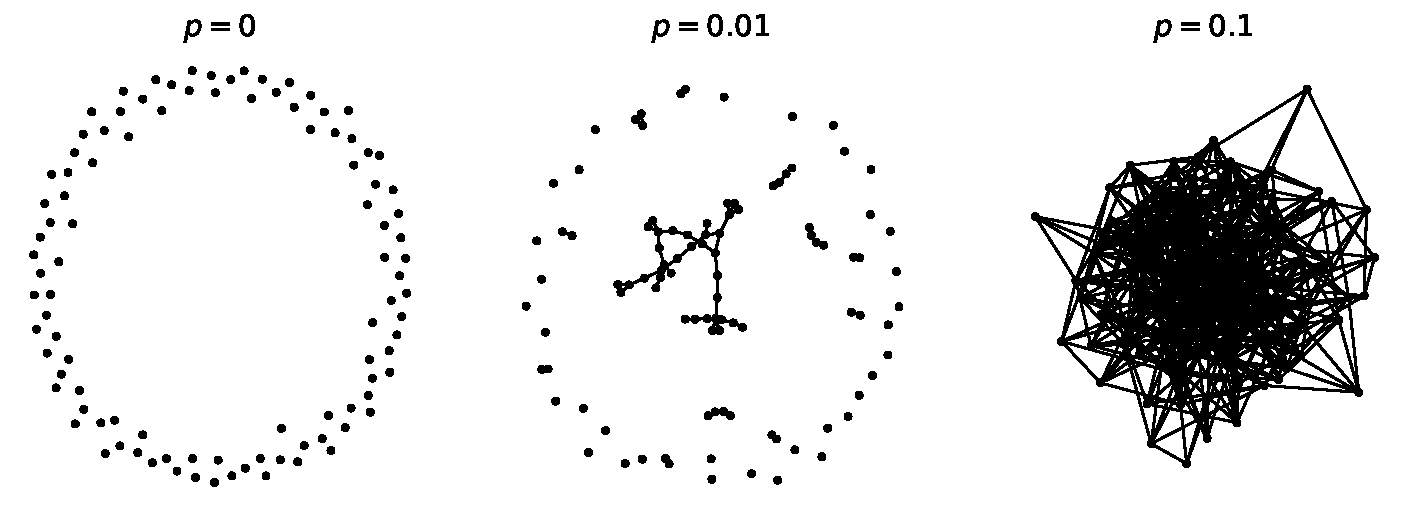
\includegraphics[width=0.9\linewidth]{figures/methodology/ERgraph}
	\caption{ER graph with $N=100$ nodes and different linking probabilities $p$.}
	\label{fig:erp}
\end{figure}

We should note that this process is stochastic. The networks $G(N, p)$ with the same parameters do not need to have the same structure; i.e. they differ in the number of links. Therefore, the single random graph is only one graph from all the possible realizations in the statistical ensemble. 

Two simple quantities that could be estimated are the average number of links and the average degree. For complete graph with $N$ nodes, number of edges is $N(N-1)/2$. As the probability of drawing every edge is $p$, the \textbf{average number of links} is simply given as 

\begin{equation}
\langle L \rangle = \frac{N(N-1)}{2}p
\end{equation}

From there, we conclude that the network's density is equal to probability $p$.
The \textbf{average degree} is approximated as: $\langle k \rangle = 2 \langle L \rangle / N $, leading to:

\begin{equation}
\langle k \rangle = (N-1)p 
\end{equation}

The \textbf{degree distribution} of ER random graph follows the binomial distribution. 

\begin{equation}
P(k) = \binom{N-1}{k}p^k(1-p)^{N-1-k}
\end{equation}

The probability that the node has degree $k$ is given with the second term $p^k$, while the probability that other N-1-k links are not created is given with the third part of the equation. Finally, there are  $\binom{N-1}{k}$ combinations for one node, to have $k$ links from $N-1$ possible links. 

The binomial distribution describes very well small networks. For larger networks, we find that they are sparse and that the average degree is much smaller than a number of nodes $\langle k \rangle << N$. In this limit, binomial distribution becomes the Poisson, which now depends only on one parameter $\langle k \rangle$

\begin{equation}
p(k) = \frac{1}{k!}e^{-\langle k \rangle}\langle k \rangle^{k}
\end{equation}

\begin{figure}[h!]
	\centering
	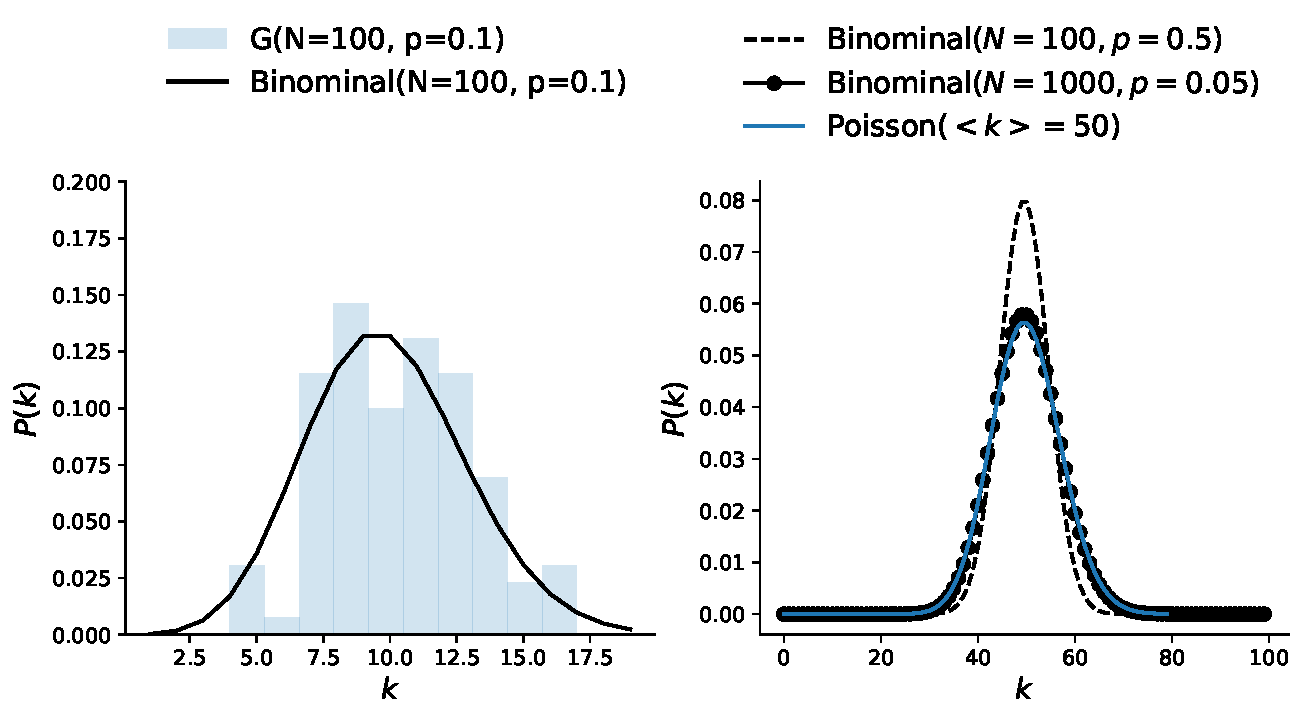
\includegraphics[width=0.9\linewidth]{figures/methodology/ER_dist}
	\caption{Degree distribution of ER graph. Degree distribution of small networks follow binominal. Larger networks are better approximated with Poison distribution, and degree distribution for fixed average degree $<k>$ becomes independent of the network size.}
	\label{fig:erdist}
\end{figure}

The random graph has a very small \textbf{average path length}, it is given as $\langle l \rangle = \frac{ln N}{ln(pN)}$ that is characteristic of many large networks. The clustering coefficient is proportional to linking probability, $\langle C \rangle = p$, so in large random networks, we find a small clustering coefficient, contrary to real-world networks. \\  %about small networks Barabasi chapter3, page 22

The figure \ref{fig:erp} shows how the network becomes more connected by increasing the linking probability $p$. When $p=0$, all nodes are disconnected. In the other limit, $p=1$, the network is fully connected. Between those two probabilities exists critical probability, where the giant component appears. The giant component is a sub-graph, which size is proportional to the network size. In other words, the network does not have disconnected components. Such change in the network is a phase transition in network connectivity and is related to percolation theory. \\

The phase transition occurs when average degree is $ \langle k  \rangle = 1$, which gives us: $p_c = \frac{1}{N-1}$, meaning that all nodes have degree larger than 1. When the $ \langle k  \rangle < 1$, the network is in the sub-critical regime where all components are small. In the critical regime, the size of the giant component is proportional to the $N^{2/3}$. In the supercritical regime, $ \langle k  \rangle > 1$, the probability of a giant component appearing is 1.

\subsection{Small-world networks}

Inspired by the idea that real-world networks are highly clustered and the average distance is small, Watts and Strogatz proposed the "small-world" model. The model starts from the regular lattice, and with rewiring links, the network starts to resemble small-world property. The procedure is the following:

\begin{itemize}
	\item At the beginning, nodes are placed on the ring lattice, and each node is connected to $k/2$ first neighbours on the left and the right side. Initially, the clustering coefficient is high, $c=3/4$. 
	\item For each link in the network, with probability $p$, we choose a random node to rewire the link. This makes long-distance nodes connect, decreasing the network's average path length. 
\end{itemize}

The model interpolates between the regular graph when the probability is $p=0$ and the random graph with $p=1$ when all links are randomly rewired. Short distances and high clustering are present in the network for the critical probabilities.

\begin{figure}[h!]
	\centering
	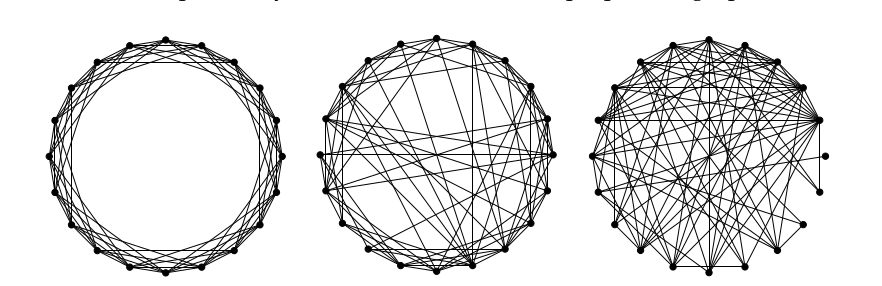
\includegraphics[width=0.9\linewidth]{figures/methodology/ws_graph}
	\caption{Watts and Strogatz graph model creation}
	\label{fig:erdist}
\end{figure}

Even though the small-world network model lacks the power-law degree distribution found in the real-world networks, it is an important model that motivated the research on random graphs. 

\subsection{Barab\' {a}si-Albert model}

The ER random graph model and WS small-world model are static models, where the number of nodes is fixed. It is one of the reasons why they can not fully explain the properties of real systems. The size of real systems does not remain constant; real networks grow. For the network, the growth means that at each time step, new nodes are added to the network. The simplest model that produces the scale-free networks is Barabasi-Albert model.

\begin{itemize}
	\item The model starts from the small number, $n_0$ randomly connected nodes, with $m_0$ links.
	\item At each time step, new node with $m$ links joins to the network. New node creates links with the nodes already present in the network, following the linking rules; i this case rules of preferential attachment. 
\end{itemize}
 
The preferential attachment is important ingredient for generating system with scale-free properties. In the real-system the linking between nodes is not random process, there exists the preference toward specific types of nodes. For example the popular web-pages can easily get more visits or it is common that already popular papers will get more citations. This effect is also called rich-get-richer or preferential attachment.

The simplest formulation of the preferential attachment model is that new nodes tend to connect with high degree nodes. The linking probability $\Pi$ is then proportional to node degree $k$:  

\begin{equation}
\Pi(k_i) = \frac{k_i}{\sum_jk_j} 
\end{equation} 

As at each time step one node arrive, we can estimate the number of nodes at the time step t, $N(t) = n_0+t$, with links $L(t) =m_0+ mt$. 

First we can calculate the evolution of network degree in time.
\begin{equation}
\frac{dk_i}{dt} = m\Pi(k_i) = m\frac{k_i}{\sum_jk_j} = m\frac{k_i}{m_0 + 2mt}
\end{equation}

Note that new node, that arrived at time point $t_i$ has degree $m$, as it links to $m$ old nodes. Solving the equation we get that at $t>t_i$, has degree that grows as square root of time, also it shows that younger nodes easily acquire larger degree. 
\begin{equation}
k_i(t) = m \left(\frac{t}{t_i}\right)^{\frac{1}{2}}
\end{equation}


Degree distribution follows power-law, and for large k is aproximated with $P(k) = k^{-\gamma}$, such that $\gamma=3$. More precisely, the degree distribution has form:

\begin{equation}
P(k) = \frac{2m(m+1)}{k(k+1)(k+2)}
\end{equation}

For large $k$ it is exactly power-law. It is also independent of the time and size of the system, meaning the emergence of stationary scale-free state. Distributions do not depend on the N. If we vary $m$ the slope of distributions is the same, but they are parallel. After re-scaling $p(k)/m^2$, they fall on the same line. 



%stationary degree dsitribution, does not depend on the system parameters, so different systems have similar behavior

As network grows nodes with larger degree becomes bigger, so we end up with few nodes with many links, called hubs. The \textbf{network diameter}, represents the maximum distance in network, $d \sim \frac{lnN}{lnlnN}$. The diameter grows slower than $lnN$, making the distances in BA model smaller than in random graph. The difference is found for large N. Knowing that BA network has hubs, that shorten the path between less connected nodes. Also, if hubs are removed from the network, network easily partition in several components, loosing its  properties. 

The \textbf{clustering coefficient} of the BA model follows $C \sim \frac{ln N^2}{N}$. It is different from clustering found in random networks, and BA networks are in general more clustered. 

The combination of the growth and preferential attachment linking is crucial for getting scale free networks. For example, eliminating the preferential attachment; in growing network with random linking, degree distribution is stationary, but it follows exponential. In contrast, the absence of growth leads to the non-stationary degree distribution. When number of nodes is fixed, while the network grows only in number of links, such that randomly chosen node $i$ connects to node $j$ according to probability $\Pi$. At the beginning, the degree distribution follows the power-law, same as in BA model. As more links are added to the network, the distribution changes it's shape, first the peak appears, while at the end network becomes complete graph, where all nodes have the same degree.  

%Absence of the preference or growth
%In summary, the absence of preferential attachment leads to a growing network with a stationary but exponential degree distribution. In contrast the absence of growth leads to the loss of stationarity, forcing the network to converge to a complete graph. This failure of Models A and B to reproduce the empirically observed scale-free distribution indicates that growth and preferential attachment are simultaneously needed for the emergence of the scale-free property.

%The BA model postulates the presence of preferential attachment. Yet, we can build models that generate scale free networks without preferential attachment. The link selection model offers the simplest mechanism that generates a scale-free network. At each time step we add new nodes to the network, we select link at random and connect the new node to one of the two nodes at the end. The higher is degree of the node, the higher is chance that node is located at the end of chosen link. The more k-degree nodes are there, the more likely is that k node is at the end of chosen link. Probability that node at the end of randomly choosen link has degree k is $q_k = Ckp_k$. The fact that bias is linear with k indicates that the link selection model builds scale-free networks. 
%Copying model can also generate scale-free networks. In each time step a new node is added to the network. To decide where it connects we randomly select node u. Then with probability $p$ new node links to $u$, otherwise with probability $1-p$ we randomly choose an outgoing link of node $u$ and link the new node to its target. The likelihood that new node connects to degree-k node is $P(k)=\frac{p}{N} + \frac{1-p}{2L}k$, the second part is equivalent in selecting a node to randomly selected link. The popularity of the copying model lies in its relevance in real systems. It is common in social networks, citation networks or even protein interactions.  in optimization, when new nodes balance conflicting criteria as they decide where to connect

%TODO \subsubsection{degree distribution derivation}
% u realnim mrezama koeficijent varira od 2 do 3

\subsection{Nonlinear preferential attachment model}

In the nonlinear preferential attachment model linking probability also depends on the node degree. The dependence is not linear and has the following a form:

\begin{equation}
\Pi(k_i) = {k_i}^{\beta}
\end{equation} 

The probability that newly added node attaches to node $i$ depends on the existing i-th node degree $k_i$, and the parameter $\beta$. When $\beta=1$, the model is BA model, where degree distribution follows the power-law. When $\beta=0$, linking probability becomes uniform; i.e. it corresponds to random network model, and degree distribution is Poisson; there is exponential decay. 

For $\beta>1$, the effects of preferential attachment are increased, leading to emergence of super-hubs. The hub-and-spoke network appear in this regime, where almost all nodes are connected to few high-degree nodes. %OVDE CITIRATI kRAPIVSKY REDNER RADOVE

On the other hand, if $\beta<1$, the model is in so called sub-linear preferential attachment regime. The linking probability is not random so degree distribution does not follow Poisson; but also the preference toward high degree nodes is too week for having the pure power-law. Instead degree distribution converge to stretched exponential.

 %While in many systems we do observe such a linear dependence, in others, like the scientific collaboration network and the actor network, preferen- tial attachment is sublinear. This nonlinear $P(k)$ is one reason the degree distribution of real networks deviates from a pure power-law. Hence for systems with sublinear  the stretched exponential (5.23) should offer a better fit to the degree distribution.


\subsection{Ageing model}

To understand how aging can impact the network structure we look into probability dependent on two parameters, nodes degree $k$ and age of node $i$ at the time point $t$ $\tau_i=(t-t_i)$, where $t_i$ is the time when node $i$ is added to the network. 
\begin{equation}
\Pi_{i}(t)\sim k_{i}\tau_{i}^{\alpha} 
\label{eq:aging}
\end{equation}

The parameter $\alpha$ controls the linking probability dependence on the nodes' age if $\alpha=0$, the ageing of nodes is disregarded. 

If $\alpha>0$ is positive, the older nodes are more likely to create connections. In this regime, the preferential attachment stays present, and the high-degree and older nodes are preferred. For very high $\alpha$, each node is connected to the oldest node in the network. The scale-free properties are present; the power-law exponent $\gamma$ deviates from $\gamma=3$. It is found that $\gamma$ ranges between $2$ and $3$. 

When $\alpha$ is negative, ageing overcomes the role of preferential attachment, and scale-free properties are lost. For significant negative $\alpha$ network becomes a chain; the youngest nodes are those who get connected. 

\begin{figure}[!ht]
	\centering
	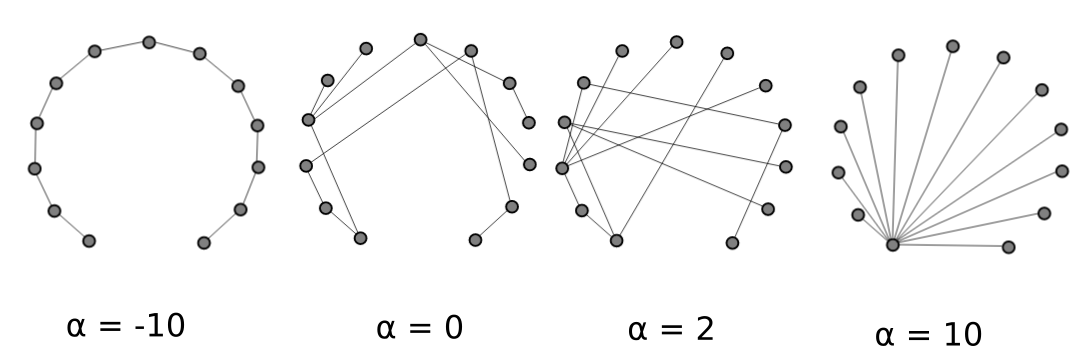
\includegraphics[width=1\linewidth]{figures/aging_nets.png}
	\caption{Aging model}
	\label{fig:aging}
\end{figure}

In the general ageing model, the non-linearity on the node degree is introduced, so this model has two tunable parameters $\alpha $ and $\beta$. The probability that a link is created between the new node and the existing node is defined as

\begin{equation}
\Pi_{i}(t)\sim k_{i}(t)^{\beta}\tau_{i}^{\alpha} 
\label{eq:1}
\end{equation}

As before, depending on model parameters network evolves to different structures \cite{hajra2004}.  
\begin{itemize}
	\item For example if we fix $\beta=1$ and $\alpha=0$ generated networks are scale-free; degree distribution is $P(k) \sim k^{-\gamma}$ with $\gamma=3$.
	\item In the case of nonlinear preferential attachment $\beta \neq 1$ and $\alpha=0$ scale-free properties disappear. 
	\item Scale-free property can be produced along the critical line $\beta(\alpha^{*})$ in the $\alpha-\beta$ phase diagram, see Figure \ref{fig:diagram}.
	
	\item For $\alpha>\alpha^{*}$ networks have \textbf{gel-like small world} behavior.
	
	\item For $\alpha<\alpha^{*}$ and near critical line $\beta(\alpha^{*})$ degree distribution has \textbf{stretched exponential} shape
	
\end{itemize}

\begin{figure}[!ht]
	\centering
	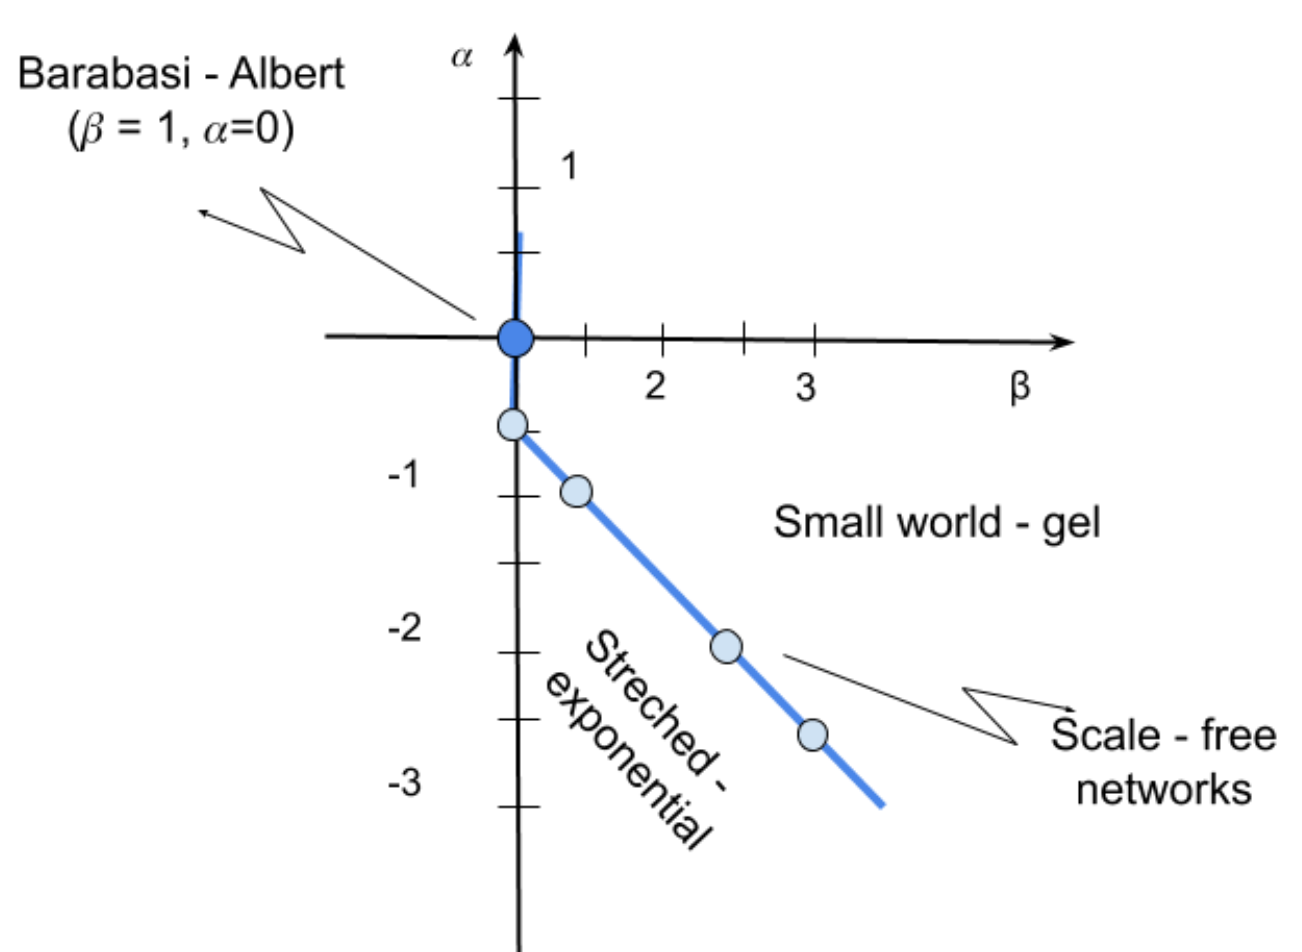
\includegraphics[width=0.5\linewidth]{Figures/diagram.png}
	\caption{Phase diagram of aging network model}
	\label{fig:diagram}
\end{figure}

\subsection{Stochastic block model}
%The network or graph is the structure of nodes and edges, where each edge connects two nodes. Nodes can be organized into groups, called communities. Identifying these hidden blocks can lead to interesting insights into the network. However, the community detection problem does not give a precise definition of what a community is. As a consequence, many approaches try to recover such structural patterns in the network \cite{martin}.



%A common definition of a community is that it is densely connected subgraph \cite{userguide}. We can find these subgraphs by optimizing an objective function, such as modularity function. It measures the difference in the number of edges between the given network and the network with the same number of nodes but randomly connected. In this approach, we try to maximize the density of connections inside a group by focusing more on assortative\footnote{Networks where nodes tend to connect with other nodes of a similar degree. Edges are more likely inside blocks than out of them.} group structures. 

%Another type of networks is the bipartite network that has two disjoint sets of nodes. The edges exist only between nodes from different sets. Networks of this class can appear in real-world data, such as users-movies preference, collaboration network for scientists and papers, etc. Application of density-based approach requires to first project bipartite network to one of its partitions and then find communities in that projection. With this, some information is lost. On the other hand, the method that is directly applicable to bipartite networks is Stochastic Block model, from which the models considered in this paper are derived. \\

Stochastic block model (SBM) is based on connection probabilities between nodes. It is a generative model which includes existence of communities. Parameters that describe SBM for network G with N nodes are:

\begin{itemize}
	\item k: number of groups
	\item group assignment vector, g: $g_i \in\{1,2..k\}$, gives the group index of node $i$.
	\item SBM matrix, $p_{k \times k}$, whose elements $p_{ij}$ are the probabilities that edges between groups $g_i$ and $g_j$ exist.
\end{itemize}

Note that nodes within one group have the same connection probabilities.

SBM can generate and describe different types of network structures. Figure \ref{fig:SBM} \cite{userguide} shows how the model matrix corresponds to resulting networks with two communities. First, for the assortative network (\ref{fig:SBM} a), diagonal elements of the matrix have higher probabilities. This indicates dense connections inside the group, just like in classic community structures. In disassortative structure, (\ref{fig:SBM} b), more connections exist between two partitions than inside them, i.e. off-diagonal elements have higher probabilities. Bipartite networks can be represented like this. 

Figure (\ref{fig:SBM} c) shows how the model represents core-periphery networks. Nodes of one block (core) are well connected with itself and with other partition (periphery). From the last case, we can note that SBM with one group is the Erdos Renyi random graph (\ref{fig:SBM} d) because all probabilities inside and between groups are equal.

\begin{figure}[!h]
	\centering
	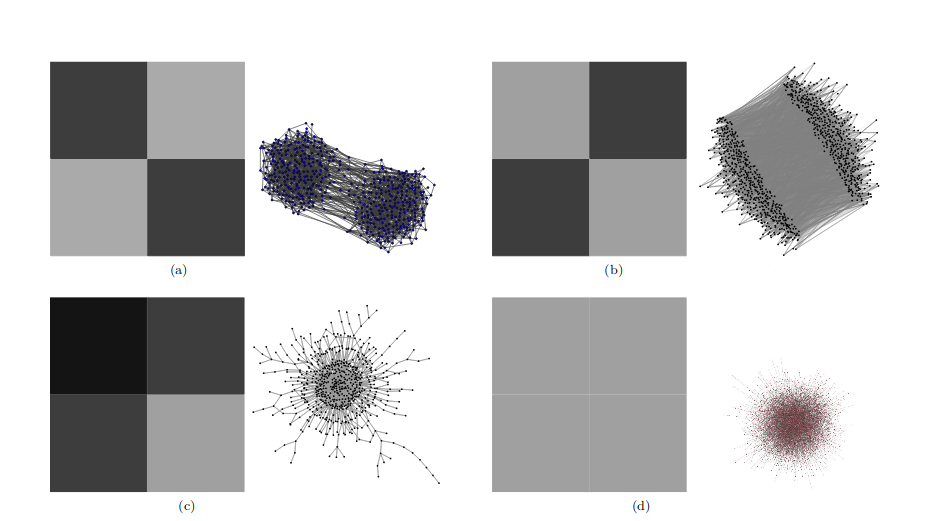
\includegraphics[width=0.5\textwidth]{Figures/structures.png}
	\caption{Stochastic Block model for different networks structures. (a) assortative. (b) dissortative. (c) core-periphery. (d) Erdos Renyi random graph.}
	\label{fig:SBM}
\end{figure}



The benefit of this model is that we can generate many networks with similar group structure. The model can fit real data, which results in finding network communities. For the given network $G$ and number of groups $k$, the best nodes partition $g$ is found by maximizing the likelihood function. Beside inferring communities, SBM has application in prediction of missing links. This simply formulated model has many variants, motivated by specific properties of real data. For example, for networks which are degree heterogeneous, there is degree corrected SBM. In some social networks, users can belong to more than one group, and this can be modelled with mixed membership SBM. Other extensions include application to bipartite, weighted network, hierarchical model, etc. Also, several algorithms for optimization of likelihood function are proposed. The overview of these versions and methods are given in \cite{comparison}. 


\newpage
\section{The properties of probability distributions}

\subsection{Poisson distribution}

Poisson distribution is exponentially bounded distribution. The property of these distributions is that they decay exponentialy or faster for high x. The largest expected value grows as $logx$, meaning that outliers representing the high x values are rate. In the network science the most common distribution is Poisson distribution, while outside the network science the most common distribution is Gaussian distribution. 

On the other hand, fat tailed distributions, long tailed or heavy tailed distributions refer to distributions whose decay for large x is slower than exponential. In this distributions events with large x value are rare but possible. 

\subsection{Power law}

The power-law distribution is defined as 

\begin{equation}
p(k) = C k^{-\gamma}
\end{equation}

where parameter $\gamma$ is an exponent of the power-law distribution while the C is the normalizing constant. 

The distribution can take both discrete and continuous values and it is defined for positive values $k>0$ so there is lower bound to the power-law function $k_{min}$ and it . For the discrete case $C=1/\zeta(\gamma, k_{min})$, while in the continuous case $C=(\gamma-1)k_{min}^{\gamma-1}$. 

The likelihood function for continuous data set is defined as 
\begin{equation}
l(k) = \prod p(k) = \prod \frac{\gamma - 1}{ k_{min}}(\frac{k_i}{k_{min}})^{-\gamma}
\end{equation}

Minimizing the loglikelihood function, exponent is calculated as $\gamma = 1+n[\sum ln \frac{k_i}{k_{min}} ]^{-1}$. 

For discrete distribution the log likelihood is $log(l) = ln\prod \frac{k_i^{-\gamma}}{\zeta(\gamma, k_{min})}$. For this equation does not exist the analytical solution, but the equation can be numericaly optimized. \\

The power-law distribution is called scale-free distribution. This is distribution that is the same on all scales. 

For example if we take power law distribution:

$$\frac{p(x)}{p(2x)} = \frac{Ax^{-\alpha}}{A(2x)^{-\alpha}} = 2^{\alpha}$$ 

This ratio is constant and does not depend on the $x$. If we take any other distribution, we'll find that this criteria is not satisfied. 

In the general form, scale free function is defined as:
$$p(bx) = g(b)p(x)$$ 
Solving this equation we get $p(x)=p(1)x^{-\alpha}$, where $\alpha=-p(1)/p^{'}(1)$, concluding that if function is self-similar, it has to be a power-law. 





\subsection{Lognormal distribution}

The variable $x$ has the lognormal distribution if the random variable $y=ln(x)$ is distributed as normal distribution. 

\begin{equation}
f(y) = \frac{1}{2\pi\sigma}e^{-(y-\mu)^2/2\sigma^2}
\end{equation}
where $\mu$ is mean, and $\sigma$ is standard deviation. The density distribution of the lognormal distribution is defined as
\begin{equation}
f(x) = \frac{1}{x \sigma \sqrt{2\pi}}e^{-(log(x)-\mu)^2 /2\sigma^2} 
\end{equation}

The lognormal distribution has finite mean $e^{\mu+1/2\sigma^2}$, and the variance $e^{2\mu+\sigma^2}(e^{\sigma^2 -1})$.  \cite{mitzenmacher2004brief}.

Despite the finite moments, the lognormal distribution can be similar to power-law distribution. If the variance of lognormal distribution is large then the probability function on log-log plot appears linear for large range of values. 

The normal distribution has property that the sum of two independent normal random variables is normal random variable with mean $\mu_1+\mu_2$, and variance $\sigma_1^2+ \sigma_2^2$. It follows that two log-normally distributed random variables also have a lognormal distribution. \cite{mitzenmacher2004brief}. 
%A lognormal distribution has finite mean and variance. .

\subsection{Power law with exponential cutoff}

The density function has the form
\begin{equation}
p(x) = C x^{-\gamma}e^{-\lambda x}
\end{equation}

where $x>0$ and $\gamma>0$. This function combines the power-law term and exponential term responsible for exponentially bounded tail. Taking the logarithm $ln(p(x)) = lnC - \gamma lnx - \lambda x$, when $x<<1/\lambda$ the second term dominates, so distribution follows te power-law, with exponent $\gamma$. Otherwise, the $\lambda x$ term domintes, resulting in exponential cutoff for high $x$. 

\subsection{Streched exponential}

the stretched exponential 

\begin{equation}
p(x) = c x^{\beta - 1}e^{-(\lambda x)^{\beta}}
\end{equation}

 the parameter $\beta$ is streching exponent determining the properties of the function $p(x)$. For $\beta=1$, the function is exponential. For $\beta<1$ it is hard to distinguish the distribution from power-law. For $\beta>1$ we have a compressed exponential function, so $x$ vary in the narrow range. \\

Whenever we encounter fat-tailed distributions, there is discussions asking which distribution offers the best fit to the data. In many systems empirical data is not sufficient to distinguish between distributions. 

\subsection{Plotting the fat-tailed distributions}

With plotting the distribution of the power-law data on the double logarithmic scale we should obtain the straight line, as $ln(p(k)) = \gamma ln(k) + c$. The tail of the distribution is noisy. As the size of the bins is constant, the density of the bins for large distribution values becomes large. To avoid the fluctuations in the tail, we can use logarithmic binning. The noise is reduced by dividing the $x$ axis into $n$ bins $b_n = c^n$, so the following bin is wider than before. For the base $c$ we can choose any value $c>1$. Similarly, the binning can take the following form $b_n = k_0\exp{(cn)}$, where $k_0$ is the minimum data point, while the $c$ is the arbitrary base. All data points between values $[b_n, b_{n+1})$ are represented with one point $p(k_n) = N_n/b_n$, where $N_n$ is number of nodes found in the bin $b_n$ and $k_n = \sum_i k_i / N_n$ is average degree of the nodes in the bin $b_n$. By this, averaging over bins in the tail, which now have more sampled points, reduces the statistical errors.

Instead of plotting the probability distribution (i.e. creating histogram), it is possible to calculate the cumulative distribution. $P(k) = \int_{x}^{\infty} p(x^{'}) dx^{'} = x^{-(\gamma-1)}$. It is also the power-law distribution with exponent $\gamma-1$. Note that for cumulative distribution it is not necessary to use log-binning. 


\subsection{The goodness-of-fit}

Minimizing the loglikelihood of function for given data, allow us to analitically or even numerically fit distributions and estimate fit parameters. Still, it does not tell us how good the fit is. 

The figure shows the distributions of three small datasets, drawn from power-law with $\gamma=2.5$, lognormal $\mu=0.3, \sigma=2$ and exponential with $\lambda=0.125$. The distributions look as straight line on the log-log plot, we could try to fit them to the power law distribution and obviosly, some model parameters could be estimated. It is not straightforward to say weather particular data really follows given distribution. Even if data follow powe-law, their observed distributions are not likely to exactly follow power-lawl there are some deviations because of the random nature of sampling procedure. 

The basic approach is to sample many synthetic data sets from a tru power-law and measure how they fluctuate from power-law form and compare results on empirical data. If empirical data are much further from power-law than syntetic one, the power-law is not plausible fit to the data. 


A standard aproach to answering this kind of questions is to use goodness-of-fit test which generate the p-value that quantifies the plausibility of the hypothesis. Measuring the distance between distributions of empirical data and the model. p-value is defined to be fraction of synthetic distances that are larger than the empirical distance. 

For measuring the distance between distributions we can use the Kolmogorov-Smirnov statistics, but in general other goodness of fit measures could be used.
The Kolmogorov Smirnov statistics is the maximum distance between the CDF of the data and the fitted model.  
\begin{equation}
D = max |S(x) - P(x)|
\end{equation}

First we fit empirical data to get model parameters, and calculate the KS statistics of this fit. Then, large number of syntetic data sets, are generated with model optimized model parameters. Then each syntetic dataset is fitted, and KS statistics is obtained relative to its own model. Then simply we count the fraction when the KS statistics of syntetic distributions is larger than in empirical data, that represents the p-value. 

If $p<0.1$ then we reject the hypothesis that this distribution describes the empirical data, otherwise the model can not be rejected. Failing to reject the hypothesis does not mean the model is correct distribution for the data. There might be other distributions that fit the data equaly good, or even better. For having accurate p-value we need large sample. For small number of syntetic distributions it is possible to have high p-value, even if the distribution is wrong model to the data. 

Using goodness of fit it is possible to calculate p-value for any distribution. For example comparing p-value of power-law fit to the p-value of trunctated power-law fit, we can conclude which one is better fit to data. If p-value for powe law is high, while for alterantive distribution it is low, we can conclude that power-law is more probable fit. 

The another method called the likelihood ratio test allows us to directly compare two distributions. The distribution with higher likelihood under epmpirical data is better fit. We can calculate the likelihood ratio, or it is easier to obtain the logarithm of likelihood ratio, because its sign determine which distribution is better fit. For given two distributions $p_1(x)$and $p_2(x)$. 

The likelihoods are defiend as $L_1=\prod_{i=1}^{n}p_1(x)$ and $L_2=\prod_{i=1}^{n}p_2(x)$, or the ratio of likelihoods as $R=\frac{L_1}{L_2} = \prod_{i=1}^{n} \frac{p_1(x)}{p_2(x)}$

Taking the logarithm, we obtain the loglikelihood ratio

\begin{equation}
\mathcal{R} = \sum_{i=1}^{n} \left[ln p_1(x) - ln p_2(x)\right]
\end{equation}

As data $x_i$ are independent, by central limit theorem their sum $\mathcal{R}$ becomes normally distributed, with expected variance $\sigma^2$. We can approximate the variance as 

$$\sigma^2 = \frac{1}{n}\sum_{1}^{n}[(l_i - l_i) - (<l>^{(1)}- <l>^{(2)})]$$

When $R>0$ the first distribution is better fit to data and when $R<0$, the other one should be chosen. When $R=0$, it is not possible to distinguish between two distributions. 

The sign of $R$ is not enough criteria to conclude which distribution is better fit. It is a random variable subject to statistical fluctuations. We need loglikelihood ratio that is sufficently positive or negative, and to be sure that its sign is not result of fluctuations.

If we are suspcted thaat the true expectation value of the loglikelihood ratio is zero, meaning that observed sign of $\mathcal{R}$ is simply product of fluctuations and an not be trusted. The probability that measured log likelihood ratio has magnitude as large or larger than observed value R is given as

\begin{equation}
p = \frac{1}{\sqrt{2\pi n \sigma^2}} \int_{-\infty}^{-|\mathcal{R}|}e^{-x^2/2n\sigma^2}dx + \int_{|\mathcal{R}|}^{\infty}e^{-x^2/2n\sigma^2}dx
\end{equation}

Here we use standard two tail hypothesis test, assuming that the null hypothesis is that $R= 0$. If p-value is larger than threshold, the sign of R is not reliable, and the test does not favor any distribution. If p is small, $p<0.1$ than it is unlikely that observed sign is obtained by chance, so we reject the null hypothesis that $R=0$. 

\section{Multiplicative processes}

Using the multiplicative processes we can generate the power-law but also the log-normal distribution. 

The lognormal distribution is generated by processes that economist Gibrat called the law of proportionate effect. 

If we start from the organism of size $S_0$. At each time step, the organism may grow or shrink,  according to random variable $\epsilon$, 

$$S_t = \epsilon_t S_{t-1}$$   

When the state of the system at time t is proportional to the state of the system at previous time step, we have the multiplicative process. The $\epsilon$ is proportionality constant that can change over time. The state of the system at time step t is determined by the product of the various $\epsilon_t$ and the initial size $S_0$ 

$$S_t = \epsilon_t S_{t-1} = \epsilon_t \epsilon_{t-1}... \epsilon_2 \epsilon_1 S_{0} $$

The $S_t$ is drawn from the log-normal distribution. If $\epsilon_t$ is drawn from the lognormal distribution, then $S_t$ also follows lognormal, as the product of lognormal distributions is again lognormal. Still, the distribution of the $\epsilon$ does not determine the distribution of the $S_jt$. 

Taking the logarithm of the equation:

$$ln(S_t) = ln(S_0) + \sum_{i=0}^{t} ln(\epsilon_i)$$

The sum of the logarithms of the $\epsilon_t$, according to the Central Limit Theorem follows the normal distribution. The CLT states that the sum of intetically distributed random variables with finite variance converge to the normal distribution. If $ln(S_t)$ is normally distributed, then $S_t$ follows the log-normal distribution.   

Using the multiplicative processes it is possible to generate the lognormal distribution. Also similar process may lead to the power-law distribution. 

In the Champernowne model, where individuals are divided into classes according to their income. The minimum income is m. People between incomes m and $\gamma m$ are in the first class, in the second class are people with income between $\gamma m$ and $\gamma^2 m $. The individuals can change their class, so it is described as the multiplicative process, but with threshold, as income can not be lower than m. For example, if we fix $\gamma=2$, and consider that with probability $p_{i,i-1}=2/3$ the change is from higher to lower class, and with probability $p_{i, i+1}=1/3$ individual goes to higher class. This process leads to the power-law distribution.


%\section{Multiplicative processes}


%Many textbooks and scientific papers deal with this topic. Some of them are very beautiful and complete and we suggest them for further reading (e.g. Mitzenmacher 2004; Newman 2005). Suppose you have an evolution process, where for example an organism transforms itself in time. As a general statement, the state S t at time t will be determined by the previous states and by the external conditions. Whenever the state of the system can be written as we have a multiplicative process. In other words, in a multiplicative process, the state of the system at time t is proportional to the state at time t-1. In biology this could represent the fact that the growth of an organism is ruled by its body mass at the previous step. In the case of city growth (Zanette and Manrubia, 1997; Manrubia and Zanette, 1998; Gabaix, 1999) this equation states that the population at a certain time step is proportional to what it was previously. In both cases the proportionality constant is given by the factor t that can change its value at any time step. Turning back to eqn 4.114 we can immediately see that the variable S t is determined by the product of the various tau where tau is between 0 and t This sum of the logarithms of the tau (under very mild conditions) is a variable following a normal distribution (regardless of the distribution of the tau ). This result comes from the application of the ‘central limit theorem’. This theorem states that, in certain very general hypotheses, the sum of identi- cally distributed random variables with finite variance is a new stochastic variable normally distributed. Therefore, if ln(S t ) is normally distributed, the variable S t is log-normally distributed. This very simple mechanism has been rediscovered and explained over and over many times since the definition of log-normal distributions in 1879 (McAlister, 1879). One of the first applications of these ideas traces back at least to the economist Gibrat (1930, 1931) who uses essentially this model under the name of proportionate effect. Using a different terminology, a somewhat similar idea was introduced at the beginning of last century for biological problems (Kapteyn 1903, 1918). With this idea we have two possible outcomes. As explained above we have true log-normal distributions that can easily be confused with power laws. This happens whenever the log-normal distribution is studied in a range of k for which $\sigma >> ln(k)$. On the other hand, a very similar situ- ation also triggers the formation of true power laws as shown in the next subsection. Powerlaws from multiplicative processes.

%\subsection {Preferential attachment}

%One of the most successful applications of multiplicative processes is given by preferential attachment. To date, this is the most successful mechanism adopted in the study of growing networks. Interestingly, the idea that we are going to explain has been independently rediscovered several times in different fields and ages. Precisely for this reason it has also been given several names. For example: Yule Process, Matthew effect, Rich gets richer, Preferential Attachment, Cumulative advantage. In the community there is some agreement (Mitzenmacher, 2004; New- man, 2005) that the first to present this idea has been G. Yule (1925) in order to explain the relative abundance of species and genera in biological taxonomic trees. As shown in Chapter 8 when considering a set of biolog- ical species we have that the classification (taxonomic) tree has scale-free properties. The null hypothesis consists in considering that the set of species arises from a common evolution. Therefore we consider one parent species and after mutation we obtain a new one that very likely can be grouped in the same genus. Every now and then though, speciated species (the new ones) can be so different from the parent one that they can form a new genus on their own (or be grouped in an existing different one). The probability of speciating will be larger for genera that are already large, since mutation rate is constant for any individual.

%This explanation allow us to focus on the two ingredients of the model. Firstly you have to invoke a certain a priori dynamics (hereafter called growth). Secondly, this dynamics selects successful elements and makes them even more successful (hereafter called preferential attachment). In detail, take a set of elements each of which is characterized by a certain number N i t . As a possible example this could be the number of different genera that have i species per genera. The set can also be a set of vertices in a graph and the number N i t can represent the number of pages whose in-degree is i. Now let us introduce a rule that introduces new elements in the set; these elements will not be shared equally between the older ones, but rather will be assigned more to those that already have many. Let us consider that N i t gives the number of vertices with certain degree i (the total

%\section{Scale-free networks}

%The study of scale ivariance has a long tradition. Among the fields where this property was analysed were the theory of critical phenomena, percolations and fractal geometry. One of the first examples considered eas the price fluctuations  of cotton in commodities market (Mandelbort, 1963). The future price can not be obtained with arbitary precision from past series., still this series have some form of regularity. The curves for daily, weakly and montly price fluctuations are statistically similar. The fact that some features are found at different time scales is typical sign of fractal behaviour. Similarly in the case of coastline lenght we find fractal behavior. If we try to measure the total lenght, the real shape is so complicated that we always miss some part. 

%Fractal behaviour might refer to different properties. In some systems scale-free structure is in shape. In this class the fractal shape can be robust, as in the case of branched patterns or electric breakdown. We say robust because these phenomena happen for varaity of external conditions. In the same class we have other systems that are more fragile, in the sense that they arise after precise tuning of some physical quantity. This is in the case of percolations and critical phenomena. Scale-free invariance may be related with dynamics or evolution of the system. The time activity of the system may display self-similar behaviour. The only sign of fractal behaviour is the mathematical form, power-law fluctuations of the time-series. 

%The self-similarity can be present in the way the different parts of a system interact with each other. This is the case with self-similar graphs and the power-law scaling appers in the distribution of topological quantities like the number of interactions per part  of the system. These phenomena are fractals in the topology. 

%\section{Scale-invariance and power laws}

%The mathematical form of self similarity is represented by powe-laws. Whenever the function $y = f(x)$ can be represented as a constant to the power of x. The physical example is elastic force, the gravitational and electrostatic force. In the case of fractals, their geometry can be identified by considering the numbe of boxes $N(\epsilon)$, of linear size $1/\epsilon$. $N(\epsilon) = \epsilon ^{-D}$, where D is called fractal dimension. D can also be defined using mass relation $M = L^ D$.

%Scale invariance is not restrected to geometry, but also appears in dynamical systems. In this case we have power-law distribution for different physical\setsecnumdepth{subsection} quantit\setsecnumdepth{subsection}ies. For example the evolution of some systems (sanspiles, number of species in the ecosystem) proceeds  with series of causally connected events whose size s is distributed as power-law. $P(s) s^{-\tau}$.

\section{Fractal analysis}

Approach to study complex systems is detecting time-series of selected variables. Some systems are characterised by periodic ot nearly periodic behaviour. In complex systems this periodic behaviour is not limited to one or two characteristic frequencies. They extend over wide spectrum and fluctuations on many time scales as well as well as broad distributions. In these cases dynamics of the system is characterized by scaling laws, which are valid over a wide range of time scales or frequencies. If dynamic of the system can be described with one scaling exponent system is monofractal, otherwise we deal with multifraactal time-series.

Rescaling of time t by a factor a may require rescaling of the time-series values $x(t)$ by factor $a^H$, to get the self-similaraity. In this case it is:
$$x(t) = a^Hx(at)$$
The Hurst exponent characterize the type of self-affinity. 

Many records do not exhibit a simple mono fractal scaling behaviour. The scaling behaviour may be more complicated , and different scaling exponents can be found for many interwoven fractal subsets of the time series. In this case the multifractal analysis must be applied. 

Two general types of multifractality exist. The multifractality due to a broad probability distribution for values of the time series, the multifractality can not be destroyed. Multifractality due to different long-term correlations of the small and large fluctuations. In this case the probability density function of the values can be regular distribution with finite moments, and the corresponding shuffled series will exhibit non-multifractal scaling as correlations are destroyed with shuffling procedure. If both kinds of multifractality are present, the shuffled series will show weaker multifractality than the original series. Multifractal analysis will reveal higher order correlations, multifractal scaling can be observed if the scaling behaviour of small and large fluctuations is different. Extreme events might be more or less correlated than typical events.  

\textbf{Long and Short-term correlations}
The time-series are presistent such that a large value is usually followed by large values and small values. Considering the increments $\delta x_i = x_i - x_{i-1}$, of self-affine series $i = 1,..,N$, with N values measured equidistant in time, so $\delta x_i$ can be either persistent, independent or anti-persistent. For the random walk with $H=0.5$ the increments are independent of each other. Persistent and anti-persistent increments, where a positive increment is likely to be followed by another positive or negative increment. 

For stationary data with constant mean and standard deviation the auto-covariance function can determine the degree of persistence. 

$$C(s) = \langle \Delta x_i \Delta x_{i+s} \rangle = \frac{1}{N-s} \sum_{i=1}^{N-s}\Delta x_i \Delta x_{i+s} $$ 

If the data are uncorrelated the $C(s)=0$. Short range correlations are described by $C(s)$ declining exponentially

$$C(s) = exp(-s/t_c)$$

such behaviour is typical for increments generated by an auto-regresive process 

$$ \Delta x_i = c\Delta x_{i-1} + \epsilon_i $$

with random uncorrelated offsets $\epsilon_i$ and $c = exp(-1/t_c)$.

For long-range correlations $\int C(s)$ diverges in the limit for long series. In practive this means that caracteristic time can not be defined because it increaseas with N. Contrary to short-range correlations, the correlation function decline as power-law 
$$C(s) = s^{-\gamma}$$
This type of behavior can be modeled by Fourier filtering techniques. Long-term correlated, behavior of $\Delta x_i$ leads to self-affine scalling beahviout characterized by $H=1-\gamma/2$. 

A direct calculation of the $C(s)$ is difficult due to present noise in the data and nonstationarity. Non-stationarities make the definition of $C(s)$ probalematic, because the average is not well defined, also $C(s)$ fluctuates around zero on large scales s, so it is not possible to obtain the correct correlation exponent $\gamma$. 

\textbf{Hurst's rescaled-range analysis}
The method called rescaled range analysis $R/S$ was proposed by the Hurst. It begins with spliting the time series $x_i$ into non overlaping segments $\nu$ of the size s, having $N_s = int(N/s)$ segments. Then is calculated the profile in each segment. 

$$Y_\nu(j) = \sum_{i=1}^{j} (x_{\nu s +i} - \langle x_{\nu s + i } \rangle _s)$$

Substracting the averages, constant trends in the data are eliminated. Finally the differences between minimum and maximum value and the standardan deviation in each segment are calculated as:

$$R_{\nu}(s) = max Y_\nu(j) - min Y_{\nu}(j)$$
$$S_{\nu}(s) = \sqrt{\frac{1}{s}\sum Y^2_{\nu}(j)}$$

Finally, the rescaled range is averged over all segments to obtain the fluctuation function F(s).

$$F_{RS}(s) = \frac{1}{N_s}\sum \frac{R_{\nu}(s)}{S_{\nu}(s)} \sim s^H$$

the H is Hurst exponent introduced in the first equation. The values of H that can be obtained by Hurst rescaled analasys are $<0H<2$. Values $H<1/2$ indicate long-term anticorrelated data, $H>1/2$ indicated long-term positively correlated data. For power-lae correlations decaying faster than $1/s$, $H=1/2$, like for uncorrelated data. 

On the other hand the standard fluctuation analysis is based on the random walk theory. For time series with zero mean, we consider the global profile, the cumulative sum:

$$Y(j) = \sum x_i$$, 
and then study how fluctuations of the profile, in a given time window of size s increase with s. 

We first divide each record of N elements into Ns non-overlaping segments of the size s, and another Ns non-overlaping segments starting from the end. Then we calculate the fluctuations in the each segment. In the standard FA we get the fluctuations just from the values of the profile at both endpoints of each segment. 

$$ F_{FA}^2(\nu, s) = [Y(\nu s) - Y((\nu +1)s)]^2$$ 

Then we can average $F^2$ over all subsequences to obtain the mean fluctuation 

$$F_2(s) = [\frac{1}{2N_s} \sum F^2(\nu,s)]^{1/2}  \sim s^H$$

For the relevant case of long-term correlations where $C(s)$ follows the power-law behaviour, $F_2(s)$ also increases by power-law. 

The fluctuation exponent is indentical with Hurst exponent for monofractal data. 

\subsection{Detrended fluctuation analysis}

DFA was introduced by Peng et al. and represents an important method for describing the non-stationary time series. As before methods it is also base on random walk theory, and the FA analysis is special case with linear detrending. 

Like in FA method first one calculates the global profile of the time series. DFA deaks with monotonous trends in a detrending procedure. This is done by establishing a polynomial trend within each segment by least-square fitting and subtracting this trend from the original profile, detrending. 

$$Y_s(j) = Y(j) - y_{\nu ,s}^{m}(j)$$

The degree of the polinomial can be varied in order to eliminate constant m=0, linear m=1, quadratic m-2, or higher order trends of the profile function. The variance of the detrended profile in each segment gives us mean-square fluctuations

$$F^2(\nu  s) = \frac{1}{s} \sum Y_s^2(j)$$

Finaly fluctioations over all segments are averaged, to obtain the mean fluctuations $F_2(s)$ as in eq. F2s, and as before, from the scaling of the fluctuating function we can determine the Hurst exponent. 

\subsection{Multifractality of the signals}

Multifractal detrended fluctuation analysis (MFDFA) \cite{kantelhardt2002, ihlen2012} to estimate multifractal Hurst exponent H(q). For given time series $\{x_i\}$ with length N, first we define global profile in the form of cumulative sum, equation \ref{eq:cumsum}, where where $\langle x\rangle $ represents average of the time series:
\begin{equation}
Y(j) = \sum_{i=0} ^j (x_i - \langle x\rangle), \quad j=1, ..., N
\label{eq:cumsum}
\end{equation}

Subtracting the mean of the time series is supposed to eliminate global trends. The profile of the signal Y is divided into $N_s = int (N/s)$ non overlapping segments of length s. If $N$ is not divisible with s the last segment will be shorter. This is handled by doing the same division from the opposite side of time series which gives us $2N_s$ segments. From each segment $\nu$, local trend $p^m_{\nu, s}$ - polynomial of order m - should be eliminated, and the variance $F^2(\nu, s)$ of detrended signal is calculated as in equation \ref{eq:var}:
\begin{equation}
F^2(\nu, s) = \frac{1}{s}\sum_{j=1}^s \left[Y(j) - p^m_{\nu, s}(j)\right]^2
\label{eq:var}
\end{equation}
Then the q-th order fluctuating function is: 
\begin{equation}
F_q(s) = \left\{\frac{1}{2N_s}\sum_{\nu}^{2N_s}\left[F^2(\nu, s)\right]^{\frac{q}{2}}\right\}^{\frac{1}{q}},  q \neq 0 \nonumber
\end{equation}

The value of $H(0)$, which corresponds to the limit $H(q), q-0$, cannot be determined directly because of the exponent diverge. Instead logarithmic averaging procedure has to be considered. 
\begin{equation}
F_0(s) = \exp \left\{\frac{1}{4N_s}\sum_{\nu}^{2N_s}ln \left[F^2(\nu, s)\right]\right\}, q=0
\end{equation}

The fluctuating function scales as power-law $F_q(s) \sim s^{H(q)}$ and the analysis of log-log plots $F_q(s)$ gives us an estimate of multifractal Hurst exponent $H(q)$.

For the monofractal time series, H(q) is independent of q, meaning that scaling is indentical for all segments, and averaging fluctuations gives indentical scaling for all values of q. If small and large fluctuations scale differently, there will be dependence of h(q) on q. Positive values of q, segments with large variance are dominant in the Fq(s), so positive q describes segments with large fluctuations. The negative values of q, H(q) describes the scaling of the segments with small fluctuations. 

Also, large fluctuations are characterized by smaller scaling exponent. 

Multifractal signal has different scaling properties over scales while monofractal is independent of the scale, i.e., H(q) is constant. 

\section{Dynamical reputation model}

Any dynamical trust or reputation model has to take into account distinct social and psychological attributes of these phenomena in order to estimate the value of any given trust metric \cite{duma2005dynamic}. First of all, the dynamics of trust is asymmetric, meaning that trust is easier to lose than to gain. As part of asymmetric dynamics, in order to make trust easier to loose the trust metric has to be sensitive to new experiences (recent activity or the absence of the activity of the agent), while still maintaining nontrivial influence of old behavior. The impact of new experiences has to be independent of
the total number of recorded or accumulated past interactions, making high levels of trust easy to lose. 
Finally, the trust metric has to detect and penalize both the sudden misbehavior and the possibly long term oscillatory behavior which deviates from community norms.

We estimate dynamic reputation of the Stack Exchange users using Dynamic Interaction Based Reputation Model (DIBRM) \cite{melnikovDynamicInteractionBasedReputation2018}. This model is based on the idea of dynamic reputation, which means that the reputation of users within the community changes continuously through time: it should rapidly decrease when there is no registered activity from the specific user in the community (reputation decay), and it should grow when frequent, constant interactions
and contributions to the community are detected. The highest growth of user's reputation is found through bursts of activity followed by short period of inactivity. 

In our implementation of the model, we do not distinguish between positive and negative interactions in the Stack Exchange communities. Therefore, we treat any interaction in the community (question, answer or comment) as potentially valuable contribution. In fact, evaluation criteria for Stack Exchange websites going through beta testing, described in SI, do not distinguish between positive and negative interactions.
The percentage of negative interactions in the communities we investigated was below 5\%, see Table 1 in SI. Filtering positive interactions would also require filtering out comments because they are not rated by the community, and that would eliminate a large portion of
direct interactions between the users of a community, which is essential for estimating their reputation.

In DIBRM, reputation value for each user of the community is estimated combining three different factors: 1) \textit{reputation growth} - the cumulative factor which represents the importance of users' activities; 2) \textit{reputation decay} - the forgetting factor which represents the continuous decrease of reputation due to inactivity; \textit{the activity period factor} - measuring the length of the period of time in which the change of reputation happened. In case of Stack Exchange communities, the forgetting factor has a literal meaning, as we can assume that past contributions provided by a user are being forgotten by active users as their attention is captured by more recent content.

In line with the the basic dichotomy of reputation dynamics, which revolves around the varying influence of past and recent behavior, DIBRM has two components: \textit{cumulative factor} - estimating the contribution of the most recent activities to the overall reputation of the user; \textit{forgetting factor} - estimating the weight of past behavior. Estimating the value of recent behavior starts with the definition of the parameter storing the basic value of a single interaction $I_{b_{n}}$. Cumulative factor $I_{c_{n}}$ then captures the additive effect of recent successive interactions. The reputational contribution $I_n$ of most recent interaction $n$ of any given user is estimated in the following way:

\begin{equation}\label{eq:ibn}
I_n = I_{b_{n}} + I_{c_{n}} = I_{b_{n}} (1+  \alpha  (1-\frac{1}{A_{n}+1}))
\end{equation}

Here, $\alpha$ is the weight of the cumulative part and $A_{n}$ is the number of sequential activities. If there is no interaction at $t_n$, this part of interactions has a value of 0. Important property of this component of dynamic reputation is the notion of sequential activities. Two successive interactions made by a user are considered sequential if the time between those two activities is less or equal to the time parameter $t_{a}$ which represents the time window of interaction. This time window represents maximum time spent by the user to make a meaningful contribution (post a question or answer or leave a comment).

\begin{equation}\label{eq:deltan}
\Delta_{n}=\frac{t_{n}-t_{n-1}}{t_{a}}
\end{equation}

If $\Delta_{n} < 1$ is less than one the number of sequential activities $A_{n}$ will increase by one, which means that the user is continuing to communicate frequently. On the other hand, large values $\Delta_{n}$ greatly increase the effect of the forgetting factor. This factor plays a major role in updating the total dynamic reputation of a user in each time step (after every recorded interaction):

\begin{equation}\label{eq:tn}
T_{n}=T_{n-1} \beta^{\Delta_{n}}+I_{n}
\end{equation}

Here, $\beta$ is the forgetting factor. In our implementation of the model, the trust is updated each day for every user irrespective of their activity status. Therefore, the decay itself is a combination of $\beta$ and $\Delta_n$: the more days pass without recorded interaction from a specific user, the more their reputation decays. Lower values of beta lead to faster decay of trust as shown on figure \ref{fig:paper_summary}.
















